% \documentclass[a4paper,10pt]{article}
\documentclass[review]{siamart}
\usepackage{url}
\usepackage{amssymb}
\usepackage{amsmath}
\usepackage{bm}
\usepackage{stmaryrd}
\usepackage{array}
\usepackage{multirow}
\usepackage{empheq}
\usepackage{enumitem}
	\setlist{nosep} % or \setlist{noitemsep} to leave space around whole list
\usepackage{color}
\usepackage{verbatim}
\usepackage{showlabels}
\usepackage{adjustbox}
\usepackage{hyperref}
\definecolor{darkgreen}{rgb}{0.0, 0.5, 0}
\usepackage[numbers,sort]{natbib}
\usepackage{cleveref}
\usepackage[belowskip=-5pt]{subcaption}
\usepackage{grffile}

\newsiamremark{remark}{Remark}
\newsiamremark{assumption}{Assumption}


% \newtheorem{lemma}{Lemma}
% \newtheorem{definition}{Definition}
% \newtheorem{theorem}{Theorem}
% \newtheorem{corollary}{Corollary}

\newcommand{\tcb}{\textcolor{blue}}
\newcommand{\tcp}{\textcolor{purple}}
\newcommand{\todo}[1]{\textcolor{red}{[TODO\@: #1]}}

\newcommand{\mdet}{\operatorname{det}}
\newcommand{\madj}{\operatorname{adj}}

% ------------------------------------------------------------------------------------ %
% ------------------------------------------------------------------------------------ %

\newcommand{\TheTitle}{Fast parallel solution of fully implict Runge-Kutta and discontinous
	Galerkin in time for numerical PDEs, Part I: the linear setting}
\newcommand{\TheAuthors}{B.S. Southworth, O. Krzysik, and W. Pazner}
\headers{Parallel solution of fully implict Runge-Kutta and DG in time I}{\TheAuthors}
\title{{\TheTitle}\thanks{This research was conducted ...
  }}

\author{Ben S. Southworth\thanks{Department of Applied Mathematics,
    University of Colorado,
    U.S.A. (\url{ben.s.southworth@gmail.com}),
    \url{http://orcid.org/0000-0002-0283-4928}}
    \and
    Oliver Krzysik
  	\thanks{School of Mathematical Sciences, Monash University,
  	Australia (\url{oliver.krzysik@monash.edu})}
  	\and
  	Will Pazner\thanks{Lawrence Livermore National Laboratory,
    U.S.A. (\url{pazner1@llnl.gov})}
}

\ifpdf%
\hypersetup{%
  pdftitle={\TheTitle},
  pdfauthor={\TheAuthors}
}
\fi

% ------------------------------------------------------------------------------------ %
% ------------------------------------------------------------------------------------ %

\begin{document}
\maketitle
\allowdisplaybreaks

\begin{abstract}

\end{abstract}


% ------------------------------------------------------------------------------------- %
% ------------------------------------------------------------------------------------- %
% ------------------------------------------------------------------------------------- %
\section{Introduction}\label{sec:intro}

% ------------------------------------------------------------------------------------- %
% ------------------------------------------------------------------------------------- %
\subsection{Fully implicit Runge-Kutta}\label{sec:intro:irk}

Consider the method-of-lines approach to the numerical solution of linear
partial differential equations (PDEs), where we discretize in space and arrive
at a system of ordinary differential equations (ODEs) in time,
%
\begin{align}\label{eq:problem}
M\mathbf{u}'(t) =  \mathcal{L}(t)\mathbf{u} + \mathbf{f}(t)
	\quad\text{in }(0,T], \quad \mathbf{u}(0) = \mathbf{u}_0,
\end{align}
%
where $M$ is a mass matrix, $\mathcal{L}(t)\in\mathbb{R}^{N\times N}$ a discrete
linear operator, and $\mathbf{f}(t)$ a time-dependent forcing function.

\footnote{Note,
PDEs with an algebraic constraint, for example, the divergence-free
constraint in Navier Stokes, instead yield a differential algebraic equation (DAE), which
requires separate careful treatment and will be the subject of a forthcoming paper.}
Then, consider time propagation using an $s$-stage Runge-Kutta scheme,
characterized by the Butcher tableaux 
%
\begin{align*}
	\renewcommand\arraystretch{1.2}
	\begin{array}
	{c|c}
	\mathbf{c}_0 & A_0\\
	\hline
	& \mathbf{b}_0^T
	\end{array},
\end{align*}
%
with Runge-Kutta matrix $A_0 = (a_{ij})$, weight vector $\mathbf{b}_0^T = (b_1,
\ldots, b_s)^T$, and quadrature nodes $\mathbf{c}_0 = (c_0, \ldots, c_s)$.

Runge-Kutta methods update the solution using a sum over stage vectors,
%
\begin{align}\label{eq:update}
\mathbf{u}_{n+1} & = \mathbf{u}_n + \delta t \sum_{i=1}^s b_i\mathbf{k}_i, \\
M\mathbf{k}_i & = \mathcal{L}\left(\mathbf{u}_n + \delta t\sum_{j=1}^s a_{ij}\mathbf{k}_j,
	t_n+\delta tc_i\right) + \mathbf{f}(t_n+\delta tc_i).\label{eq:stages}
\end{align}
%
Expanding, solving for the stages $\mathbf{k}$ can then be expressed as the
solution of the block linear system,
%
\begin{align}\label{eq:k0}
\left( \begin{bmatrix} M  & & \mathbf{0} \\ & \ddots \\ \mathbf{0} & & M\end{bmatrix}
	- \delta t \begin{bmatrix} a_{11}\mathcal{L}_1 & ... & a_{1s}\mathcal{L}_1 \\
	\vdots & \ddots & \vdots \\ a_{s1}\mathcal{L}_s & ... & a_{ss} \mathcal{L}_s \end{bmatrix} \right)
	\begin{bmatrix} \mathbf{k}_1 \\ \vdots \\ \mathbf{k}_s \end{bmatrix} 
& = \begin{bmatrix} \mathbf{f}_1 \\ \vdots \\ \mathbf{f}_s \end{bmatrix},
\end{align}
%
where $\mathcal{L}_i := \mathcal{L}(t_n+\delta tc_i)$. Primarily this paper
focuses on spatial operators that are independent of time; however, some of
the results hold for commuting operators, such as may arise in, for example,
a time-dependent reaction term, so for now we maintain this generality.

The difficulty in fully implicit Runge-Kutta methods (which we will denote IRK) lies in
solving the $Ns\times Ns$ block linear system in \eqref{eq:k0}. This paper focuses on the
parallel simulation of numerical PDEs, where $N$ is typically very large
and $\mathcal{L}$ is highly ill-conditioned. In such cases, direct
solution techniques to solve \eqref{eq:k0} are not a viable option, and fast, parallel 
iterative methods must be used. However, IRK methods are rarely employed in practice due
to the difficulties of solving \eqref{eq:k0}. Even for relatively simple
parabolic PDEs where $\mathcal{L}$ is symmetric positive definite (SPD), \eqref{eq:k0}
instead yields a large nonsymmetric system with significant block coupling. For
nonsymmetric systems $\mathcal{L}$ that already have variable coupling, fast iterative
methods are even less likely to yield acceptable performance in solving \eqref{eq:k0}.

% ------------------------------------------------------------------------------------- %
% ------------------------------------------------------------------------------------- %
\subsection{Discontinuous Galerkin in time}\label{sec:intro:dg}

Another field that has seen growing interest recently for numerical PDEs is discretizing
in time using finite elements, rather than standard ODE techniques. Some of the more
interesting features of using finite-elements in time is the natural ability to handle
time-dependent domains, unstructured meshes in space-time, and adaptive mesh
refinement in space and time. However, for so-called slab-based meshing in time with
discontinuous Galerkin finite elements, where
the time domain is discretized using spatial slabs (that is, the same time step is
applied to the entire spatial domain), the resulting linear systems that must be
solved for each time step take the same structure as \eqref{eq:k0} (for example,
see \cite{hn}). A handful of works have looked at linear solvers for such
discretizations, primarily for parabolic problems, including block preconditioning
approaches \cite{exh,8jp,27n}, and direct space-time multigrid methods 
\cite{gander2016analysis}.

Although this paper focuses on fully implicit Runge-Kutta, the algorithms developed
here can be directly applied to discontinuous Galerkin discretizations in time on
fixed slab-based meshes. In fact, the principles used in this paper are similar
to those used in \cite{exh} for space-time DG discretizations of linear parabolic
problems, and some of the theory derived therein...

but here we consider much more general settings, including both
non-parabolic and nonlinear problems.

% ------------------------------------------------------------------------------------- %
% ------------------------------------------------------------------------------------- %
\subsection{Outline}\label{sec:intro:outline}

This paper develops fast, parallel preconditioning techniques for the solution of
fully implicit Runge-Kutta methods in numerical PDEs. Although we focus on implicit
Runge-Kutta, the techniques developed extend naturally to DG
finite elements in time as well, as discussed in \Cref{sec:intro:dg}. 
First, \Cref{sec:intro:hist} provides background on why IRK methods are desirable
over the simpler and more commonly used DIRK methods, and also provides a
historical context for the preconditioners developed in this work.
\Cref{sec:intro:stab} then briefly discusses stable integration from
a method-of-lines perspective and introduces two key elements that will be
used throughout the paper. 

\Cref{sec:solve} introduces an effective method to solve for the IRK update
\eqref{eq:update} directly for linear operators $\mathcal{L}$ that are independent of time,
such as those that typically arise in linear PDEs. The new method effectively
requires the preconditioning of $s$ real-valued matrices along the lines of
$\eta M - \delta t\mathcal{L}$, for some $\eta > 1$, and is easily implemented
using existing preconditioners and parallel software libraries. 
In contrast to other works that have considered the preconditioning of \eqref{eq:kron1},
the proposed algorithm here (i) is amenable to short-term Krylov recursion (conjugate
gradient (CG)/MINRES) if $\eta M - \mathcal{L}$ is, and (ii) only operates on the solution,
thus not requiring the storage of each stage vector. Theory is developed
that guarantees rapid convergence of GMRES and CG under basic assumptions
on stability from \Cref{sec:intro:stab}. Numerical results for the
linear setting are provided in \Cref{sec:numerics}, demonstrating
up to 10th-order accuracy using Gauss integration with a variety of problems
and preconditioners. In addition, by using the new method with 2-stage Gauss
integration, we are able to halve the number of AMG preconditioning iterations
necessary to obtain 4th-order accuracy on an advection-diffusion example
compared with standard 4th-order SDIRK schemes.

% ------------------------------------------------------------------------------------- %
% ------------------------------------------------------------------------------------- %
\subsection{Why fully implicit and previous work}\label{sec:intro:hist}

\todo{Add citations}
Although difficult to solve, there are a number of desirable properties of IRK schemes,
particularly in terms of accuracy and stabillity (\todo{why stability?}).
In practice, people typically use
diagonally implicit Runge-Kutta (DIRK) methods, where $A_0$ is lower triangular, or
singly implicit Runge Kutta (SIRK) methods, where $A_0$ has exactly one positive real
eigenvalue. For such schemes, the solution of \eqref{eq:k0} only requires $s$ linear
solves along the lines of $M - \delta ta_{ii}\mathcal{L}_i$. Unfortunately, SIRK and DIRK
schemes suffer from stage-order one (stage-order two with one explicit stage; see
EDIRK methods), and for
stiff nonlinear PDEs, the observed global order of accuracy in practice can be limited to
$\approx \min\{ p, q+1\}$, for integration order $p$ and stage-order $q$. Thus, even
a 6th-order DIRK method may only yield 2nd-order accuracy. Accuracy is even worse for
index-2 DAEs, where the algebraic variable is limited to first-order accuracy with
DIRK methods \todo{cite Hairer} (which will be addressed as a follow-up to this paper). 
In contrast, IRK methods yield high stage order and, thus, formally high-order accuracy
on stiff, nonlinear problems, and even index-2 DAEs. Furthermore, for less stiff
problems, IRK methods can yield accuracy as high as order $2s$ for an $s$ stage method,
compared with a maximum of $s$ or $s+1$ for SDIRK methods with reasonable stability
properties \cite[Section IV.6]{hairer96}.

One simplification for using IRK methods in practice is to assume $\mathcal{L}_i =
\mathcal{L}_j$ for all $i,j$, that is, $\mathcal{L}$ has no dependence on time. Such
an assumption is natural for linear problems with no time-dependence in the spatial
differential components, or when applying a simplified Newton method to nonlinear
problems, where the Jacobian is only evaluated at one time-point per outer RK time
step. Either case yields a simplified form of \eqref{eq:k0} that can be expressed in
Kronecker product form,
%
\begin{align}\label{eq:kron1}
(I\otimes M - \delta t A_0\otimes \mathcal{L})\mathbf{k} & = \mathbf{f},
\end{align}
%
where $\mathcal{L}$ is a fixed real-valued spatial operator or Jacobian.

% To avoid complex arithmetic, one can pose each complex
% system as a real $2\times 2$ block system,
% Because eigenvalues come in conjugate pairs, we will
% instead consider inverting conjugate pairs $(\overline{\lambda_i}I - \mathcal{L})^{-1}
% = \overline{(\lambda_iI - \mathcal{L})^{-1}}$, and thus the same solver/preconditioner
% could be used for conjugate pairs of eigenvalues \todo{cite}. However, this does not
% solve the underlying problem of constructing complex solvers/preconditioners in
% practice. 

Many papers have considered the solution of \eqref{eq:kron1}. In 1976,
Butcher \cite{butcher76} used the Jordan normal form, $A_0 = U_0L_0U_0^{-1}$, where
$L_0$ is lower triangular with eigenvalues of $A_0$ on the diagonal, to transform
\eqref{eq:kron1} to the problem
$(I\otimes M - \delta t L_0\otimes \mathcal{L})(U_0^{-1}\otimes I)\mathbf{k} =
(U_0\otimes I)^{-1}\mathbf{f}$, where the inner operator is now block lower triangular.
Such a transformation reduces the solution of an $Ns\times Ns$ system to $s$ linear
systems of size $N\times N$ in a block forward solve. The downside is that
IRK schemes with greater accuracy and stability than DIRK schemes have at most one real
eigenvalue \cite{hairer96,butcher2016numerical}.
Thus, for IRK methods such as Gauss or Radau integration, the original real-valued
system is transformed into a set of smaller but primarily complex systems. There are various
ways to handle the complex systems,
but for numerial PDEs, the overhead in computational cost and implementation is typically
too high to make the transformation a practical approach.  

Published shortly after (and independently from) Butcher, Bickart proposed a similar
way to invert \eqref{eq:kron1} \cite{bickart77}. If we define $Q_s(x)$ as
the characteristic polynomial of $A_0$, then the inverse of \eqref{eq:kron1} can be computed
via a specific set of matrix-vector multiplications in addition to the action of
$Q_s(\mathcal{L})^{-1}$.
In principle this is similar to Butcher's result, as one can invert
$Q_s(\mathcal{L})$ by inverting 
each term in the factored polynomial, $(\mu_1 I-\mathcal{L})^{-1}$,
$(\mu_2 I-\mathcal{L})^{-1}$, ..., for eigenvalues $\{\mu_i\}_{i=1}^s$ of $A_0$.
Although Bickart's paper received less attention than Butcher's over time (currently $2.5\times$
less citations), the polynomial form provides a more natural way to handle complex eigenvalues,
particularly for numerical PDEs in the modern high-performance computing landscape,
where direct LU inverses are rare and most linear systems are solved via preconditioning
and/or Krylov methods. We present a similar result in \Cref{lem:inv} and use this to
develop an effective preconditioning for linear problems in \Cref{sec:solve:prec}.

Because significant research has been done on IRK methods, it is worth briefly
reviewing some of the literature to put this work in context. In the field of time
integration, SIRK and DIRK methods overcome the difficulty of solving IRK methods
\cite{alexander1977diagonally,norsett1976runge}.
In \cite{orel91}, it is shown that in considering RK methods with all real eigenvalues
(wherein the Butcher transformation \cite{butcher76} remains real-valued), the best
approximation to exponential is obtained by having all eigenvalues equal (SIRK
methods \cite{norsett1976runge}).
Although SIRK methods offer some advantages over DIRK methods, they generally lack
the favorable stability and accuracy of IRK methods \cite{burrage82,orel91}. ESIRK methods
use one explicit stage and can offer stage-order two \cite{butcher00} (one higher
than standard SIRK methods), which provide an improved practical option, but still
lack the robustness of fully implicit methods.




% Simplified newton scheme uses fixed Jacobian for all stages
% Single step Newton (Cooper (83/90), Gonzales-Pinto (95/97)
% ---------------- ODEs and LU ---------------- %
% Varah (79):
% \begin{itemize}
% 	\item Much better description of Butcher's method. Transforms coordinate system of Jacobian tensor.
% 	Still relies on this tensor structure to do said transformation. 
% 	\item Transforms Jacobian to Hessenberg form to avoid repeated action computing LU of a shifted 
% 	Jacobian.
% \end{itemize}

% Cooper:
% \begin{itemize}
% 	\item (83,90,93): develops single Newton scheme using SOR or various matrix splittings,
% 	applied to ODEs. This is a single-step
% 	Newton method, where the actual Jacobian solve is replaced with an SOR iteration. Here, Butcher
% 	matrix A is replaced with an approximate matrix with one positive real eigenvalue. 
% \end{itemize}

% Pinto:
% \begin{itemize}
% 	\item (95) Mostly ODEs, do consider 1d-space-1d-time burgers on a very small grid. 
% 	\item (96) additional iteration of single Newton, makes it quasi-Newton like. 
% 	\item (01) Analysis of single Newton (SOR) w/ simplified Newton for higer order. 
% \end{itemize}

% Brugano (2014) and Antonana (2018)
% \begin{itemize}
% 	\item New splitting and IRK techniques for Hamiltonian problems where conservation is
% 	important. Used for ODEs. 
% \end{itemize}


% % ---------------- PDEs ---------------- %

% Jay
% \begin{itemize}
% 	\item 1999: develops a preconditioning technique based on W-transformation. W-transformation
% 	yields a real-valued block-tridiagonal matrix. This can be solved using LU, but the inverses
% 	have a recursive nature (like Schur complements). They precondition w/ an approximate LU,
% 	where each formal inverse in LU is approximated, $H_i = I +
% 	\zeta_{i-1}^2\delta t^2 JH_{i-1}^{-1}J$, for Jacobian $J$ and matrix $H$ that must be
% 	inverted in LU, with $\hat{H}_i = I - \gamma_i\delta tJ$, for a certain \gamma_i$. 

% 	\item 2000: Analyzes simplified Newton to approximate time-dependent Jacobian with
% 	Kronecker product form. 
% \end{itemize}

% Houwen 
% \begin{itemize}
% \item TRIANGULARLY(1997): Uses crout factorization to pick lower triangular preconditioner.
% \item Paralell(97): 
% \end{itemize}

% Hoffman 
% \begin{itemize}
% \item (97): Also uses triangular preocnditioner on the nonlinear level.
% \end{itemize}


% Van Lent (2004)
% \begin{itemize}
% 	\item Multigrid for IRK?
% \end{itemize}

% Staff \& Mardal (2006)
% \begin{itemize}
% 	\item One of first paper to consider preconditioning the fully implicit RK system.
% 	Use block Jacobi and block lower triangular preconditioners for the diffusion equation.
% 	Use multigrid V-cycles and full Newton time-dependent Jacobian. Upper triangular is
% 	bad compared to block Jacobi and lower triangular (this has appeared elsewhere in
% 	literature -- $A_0$ is dominant in lower triangular part -- Crout factorization
% 	in I think Messina or Van der Houwen; comes up again in Brugano (2015)).
% \end{itemize}
% Mardal (2007)
% \begin{itemize}
% 	\item Analyze block-diagonal preconditioners in a Sobolev setting, demonstrate
% 	conditioning of the preconditioned operator to be optimal in the independent of
% 	$h$ sense. Use multigrid w/ diffusion as example. 
% \end{itemize}
% Nilssen (2011)
% \begin{itemize}
% 	\item Analogous to above, Sobolev analysis for block-diagonal preconditioning
% 	applied to the bidomain equations.
% \end{itemize}

% Xie (2011)
% \begin{itemize}
% 	\item Proposes a modified simplified Newton for the time-dependent cast, where the Jacobian is
% 	formed based on a least squares approximation to the true RK coefficients, evaluating all entries
% 	at a single time point. In example problems, modified Jacobian typically converged faster
% 	than simplified (evaluated at previous time step), up to 2x less iterations/time. 
% \end{itemize}

% Hao Chen:
% \begin{itemize}
% 	\item (2014) Develops a splitting iterative method to precondition IRK matrices, similar to ADI schemes.
% 	Proves that for definite spatial operators and Butcher matrices (that is, eignvalues have positive
% 	or negative real parts), $\rho(T) < 1$, where $T$ is the fixed-point iteration matrix. Look at 
% 	diffusion equation with IRK and BVMs.
% 	\item (2016) Analogous to above, extended to wave equation.
% \end{itemize}

% Pazner
% \begin{itemize}
% 	\item
% \end{itemize}

% \begin{itemize}
% 	\item if the underlying IRK methods are A-stable, irreducible, and have invertible coefficientmatrixA, such as Gauss, RadauIIA, and LobattoIIIC (cf., e.g., [Hairer]), then the real partsof the eigenvalues ofAare positive,
% 	\item One benefit of this method is ability to use PCG or GMRES on smaller system, not full system. 
% \end{itemize}

% ------------------------------------------------------------------------------------- %
% ------------------------------------------------------------------------------------- %
\subsection{A preconditioning framework and stability}\label{sec:intro:stab}

Throughout the paper, we use the reformulation used in, for example,
\cite{pazner17}, where we can pull an $A_0\otimes I$ out of the
fully implicit system in \eqref{eq:k0}, yielding the equivalent problem
%
\begin{align}\label{eq:keq}
\left( A_0^{-1}\otimes M - \delta t \begin{bmatrix} \mathcal{L}_1  & \\ & \ddots \\ && \mathcal{L}_s\end{bmatrix}\right)
	(A_0\otimes I)	\begin{bmatrix} \mathbf{k}_1 \\ \vdots \\ \mathbf{k}_s \end{bmatrix} 
& = \begin{bmatrix} \mathbf{f}_1 \\ \vdots \\ \mathbf{f}_s \end{bmatrix}.
\end{align}
%
The off-diagonal block coupling in \eqref{eq:keq} now consists of mass matrices
rather than differential operators, which makes the analysis and solution more
tractable.\footnote{For some of the methods introduced in this paper,
more-or-less equivalent algorithms can be developed
for \eqref{eq:k0} (that is, without extracting $A_0\otimes I$). However, 
the derivation and analysis therein is more difficult, and the resulting
algorithms offer no clear benefits over the presented methods.}
The algorithms developed here depend on the eigenvalues of $A_0$ and
$A_0^{-1}$, leading to our first assumption.
%
\begin{assumption}\label{ass:eig}
Assume that all eigenvalues of $A_0$ have positive real part.
\end{assumption}
%
Recall that if an IRK method is A-stable, irreducible, and $A_0$ is invertible
(which includes Gauss, RadauIIA, and LobattoIIIC integration, among others), 
then \Cref{ass:eig} holds \cite{hairer96}; that is, this assumption is 
straightforward to satisfy in practice. 

Stability must be taken into consideration when applying ODE solvers within a
method-of-lines approach to numerical PDEs. The Dalhquist test problem extends
naturally to this setting, where we are interested in the stability of the
linearized operator $\mathcal{L}$, for the ODE(s)
$\mathbf{u}'(t) = \mathcal{L}\mathbf{u}$, with solution $e^{t\mathcal{L}}\mathbf{u}$.
A necessary condition for stability is that the eigenvalues of $\mathcal{L}$
lie within distance $\mathcal{O}(\delta t)$ of the region of stability for 
the Runge-Kutta scheme of choice (e.g., see \cite{reddy92}). Here we are
interested in implicit schemes and, because the majority of implicit Runge-Kutta schemes
used in practice are A- or L-stable, an effectively necessary condition for
stability is that the eigenvalues of $\mathcal{L}$ be nonpositive. For
normal operators, this requirement ends up being a necessary and sufficient
condition for stability, as the eigenvectors form an orthogonal basis. 

For non-normal or non-diagonalizable operators, the analysis is more complicated.
One of the best known works on the subject is by Reddy and Trefethen \cite{reddy92},
where necessary and sufficient conditions for stability are derived as the
$\varepsilon$ pseudo-eigenvalues of $\mathcal{L}$ being within 
$\mathcal{O}(\varepsilon) + \mathcal{O}(\delta t)$ of the stability region
as $\varepsilon,\delta t\to 0$. Here we relax this assumption to something
that is more tractable to work with by noting that the $\varepsilon$
pseudo-eigenvalues are contained within the field-of-values to
$\mathcal{O}(\varepsilon)$ \cite[Eq. (17.9)]{trefethen2005spectra},
where the field of values are defined as
%
\begin{align}\label{eq:fov}
W(\mathcal{L}) := \left\{ \langle \mathcal{L}\mathbf{x},\mathbf{x}\rangle \text{ : }
	\|\mathbf{x}\| = 1 \right\}.
\end{align}
%
This motivates the following assumption for the analysis done in this paper.
%
\begin{assumption}\label{ass:fov}
Let $\mathcal{L}$ be the linearized spatial operator representing a single
time step. Assume $W(\mathcal{L}) \leq 0$.
\end{assumption}
%
It should be noted that the field-of-values have an additional connection
to stability. From \cite[Theorem 17.1]{trefethen2005spectra}, we have that
$\|e^{t\mathcal{L}}\|\leq 1$ for all $t\geq 0$ i.f.f. $W(\mathcal{L}) \leq 0$.
This is analogous to the ``strong stability'' discussed by Leveque 
\cite[Chapter 9.5]{leveque2007finite}, as opposed to the weaker (but still
sufficient) condition $\|e^{t\mathcal{L}}\|\leq C$ for all $t\geq 0$ and
some constant $C$. In practice, \Cref{ass:fov} is likely to hold when
simulating numerical PDEs, and in \Cref{sec:solve:prec}, it is proven that
\Cref{ass:eig} and \ref{ass:fov} provide sufficient conditions to guarantee
fast Krylov convergence of the proposed methods.

% ------------------------------------------------------------------------------------- %
% ------------------------------------------------------------------------------------- %
% ------------------------------------------------------------------------------------- %
\section{Fast parallel preconditioning}\label{sec:solve}

For ease of notation, let us scale both sides of the \eqref{eq:keq} by a
block-diagonal mass matrix inverse and let
%
\begin{equation*}
\widehat{\mathcal{L}}_i := \delta t M^{-1}\mathcal{L}_i,
\end{equation*}
%
for $i=1,..,s$. Note the time step $\delta t$ for the given Runge-Kutta step is now
included in $\widehat{\mathcal{L}}_i$. Now let $\alpha_{ij}$ denote the $ij$-element
of $A_0^{-1}$ (assuming $A_0$ is invertible). Then, solving \eqref{eq:k0} can be 
effectively reduced to inverting the operator\footnote{Note, there are a number of
methods with one explicit stage preceded or followed by several fully implicit and
coupled stages. In such cases, $A_0$ is not invertible, but the explicit stage can
be eliminated from the system (by doing an explicit time step). The remaining operator
can then be reformulated as in \eqref{eq:keq}, and the inverse that must be applied
takes the form of \eqref{eq:k1} but based on a principle submatrix of $A_0$.}
%
\begin{align}\nonumber
\mathcal{M}_s & := A_0^{-1}\otimes I - \begin{bmatrix} \widehat{\mathcal{L}}_1  & \\ & \ddots \\ && \widehat{\mathcal{L}}_s\end{bmatrix} \\
& = \begin{bmatrix} \alpha_{11}I - \widehat{\mathcal{L}}_1 & \alpha_{12}I & ... & \alpha_{1s}I \\
	\alpha_{21}I & \alpha_{22}I - \widehat{\mathcal{L}}_2 & & \alpha_{2s}I \\
	\ddots & & \ddots & \vdots \\ \alpha_{s1}I & ... & \alpha_{s(s-1)}I & \alpha_{ss}I - \widehat{\mathcal{L}}_s \end{bmatrix}.
	\label{eq:k1}
\end{align}
%

We proceed by deriving a closed form inverse \eqref{eq:k1}, demonstrating
how the Runge-Kutta update in \eqref{eq:update} can then be performed directly
(without forming and saving each stage vector), and developing a preconditioning
strategy to apply this update using existing fast, parallel preconditioners.
In \Cref{sec:solve:gamma}, analysis proves that with the right choice
of constant in the preconditioner, the preconditioned operator has condition
number $<9$, independent of problem size, order, and number of stages.

% ------------------------------------------------------------------------------------- %
% ------------------------------------------------------------------------------------- %
\subsection{An inverse and update for commuting operators}\label{sec:solve:inv}

This section introduces a result similar to Bickart's \cite{bickart77},
but using a different framework and generalized to hold for commuting
operators. If $\widehat{\mathcal{L}}_i=\widehat{\mathcal{L}}_j$ for all $i,j$, we show that
the inverse of \eqref{eq:k1} can be expressed in terms of $P_s(\widehat{\mathcal{L}})^{-1}$,
where $P_s(\widehat{\mathcal{L}})$ is the characteristic polynomial of $A_0^{-1}$. Note, we
consider $\mathcal{M}_s$ as a matrix over the commutative ring of linear combinations of
$\{I, \mathcal{L}\}$, and the determinant and adjugate referred to in
\Cref{lem:inv} are defined over matrix-valued elements rather than scalars.

%
\begin{lemma}\label{lem:inv}
Let $\alpha_{ij}$ denote the $(i,j)$th entry of $A_0^{-1}$ and assume
$\{\widehat{\mathcal{L}}_i\}_{i=1}^s$ are commuting operators. Define $\mathcal{M}_s$
% \begin{align*}
% \mathcal{M}_s := \begin{bmatrix} \alpha_{11}I - \widehat{\mathcal{L}}_1 & \alpha_{12}I & ... & \alpha_{1s}I \\
% 	\alpha_{21}I & \alpha_{22}I - \widehat{\mathcal{L}}_2 & & \alpha_{2s}I \\
% 	\ddots & & \ddots & \vdots \\ \alpha_{s1}I & ... & \alpha_{s(s-1)}I & \alpha_{ss}I - \widehat{\mathcal{L}}_s \end{bmatrix},
% \end{align*}
as in \eqref{eq:k1}.
Let det$(\mathcal{M}_s)$ be the determinant of $\mathcal{M}_s$ (in this case a block-diagonal
matrix) and let adj$(\mathcal{M}_s)$ be the adjugate of $\mathcal{M}_s$. Then, $\mathcal{M}_s$
is invertible if and only if det$(\mathcal{M}_s)$ is invertible, and
\begin{align*}
\mathcal{M}_s^{-1} = \textnormal{det}(\mathcal{M}_s)^{-1}\textnormal{adj}(\mathcal{M}_s).
\end{align*}
%

Now, suppose $\widehat{\mathcal{L}}_i = \widehat{\mathcal{L}}_j$ for all $i,j$, and let $P_s(x)$ be the
characteristic polynomial of $A_0^{-1}$. Then,
\begin{align*}
\mathcal{M}_s^{-1} = \textnormal{diag}(P_s(\widehat{\mathcal{L}})^{-1})\textnormal{adj}(\mathcal{M}_s),
\end{align*}
where ``diag'' indicates a block diagonal matrix, with diagonal blocks given by $P_s(\widehat{\mathcal{L}})^{-1}$.
\end{lemma}
%
\begin{proof}
Notice in \eqref{eq:k1} that if $\widehat{\mathcal{L}}_i$ and $\widehat{\mathcal{L}}_j$ commute for all $i,j$,
then $\mathcal{M}_s$ is a matrix over the commutative ring of linear combinations
of $I$ and $\{\widehat{\mathcal{L}}_i\}$. Let adj$(\mathcal{M}_s)$ denote the matrix adjugate. A
classical result in matrix analysis then tells us that
%
\begin{align*} 
\textnormal{adj}(\mathcal{M}_s)\mathcal{M}_s = \mathcal{M}_s\textnormal{adj}(\mathcal{M}_s)
	= \textnormal{det}(\mathcal{M}_s)I.
\end{align*}
%
Moreover, $\mathcal{M}_s$ is invertible if and only if if the determinant of $\mathcal{M}_s$
is invertible, in which case $\mathcal{M}_s^{-1} := $ det$(\mathcal{M}_s)^{-1}$adj$(\mathcal{M}_s)$
\cite[Theorem 2.19 \& Corollary 2.21]{brown1993matrices}
For the case of time-independent operators ($\widehat{\mathcal{L}}_i=\widehat{\mathcal{L}}_j$), notice that
$\mathcal{M}_s$ takes the form $A_0^{-1} - \widehat{\mathcal{L}}I$ over the commutative ring defined
above. Analogous to a scalar matrix, the determinant of $A_0^{-1} - \widehat{\mathcal{L}}I$ is the
characteristic polynomial of $A_0^{-1}$ evaluated at $\widehat{\mathcal{L}}$.
\end{proof}
%

Returning to \eqref{eq:keq}, we can express the direct solution for the set of all
stage vectors ${\mathbf{k}} = [\mathbf{k}_1; ...; \mathbf{k}_s]$ as
%
\begin{align*}
\mathbf{k} &:= \textnormal{det}(\mathcal{M}_s)^{-1}
	(A_0^{-1}\otimes I)\textnormal{adj}(\mathcal{M}_s)\mathbf{f},
\end{align*}
%
where $\mathbf{f} = [\mathbf{f}_1; ...; \mathbf{f}_s]$ (note that
$A_0\otimes I$ commutes with $\textnormal{det}(\mathcal{M}_s)^{-1}$). Excusing the slight
abuse in notation, let $\textnormal{det}(\mathcal{M}_s)^{-1}$ now denote just the diagonal
block (rather than a block-diagonal matrix). The Runge-Kutta update is then given by
%
\begin{align}\nonumber
\mathbf{u}_{n+1} & = \mathbf{u}_n + \delta t\sum_{i=1}^s b_i{\mathbf{k}}_i \\
& = \mathbf{u}_n + \delta t\textnormal{det}(\mathcal{M}_s)^{-1}
	(\mathbf{b}_0^TA_0^{-1}\otimes I)\textnormal{adj}(\mathcal{M}_s)\mathbf{f}.\label{eq:update2}
\end{align}
%

\begin{remark}[Implementation \& complexity]
The adjugate consists of linear combinations of $I$ and $\widehat{\mathcal{L}}$, and an
analytical form can be derived for an arbitrary $s\times s$ matrix, where
$s\sim\mathcal{O}(1)$.
% Computing this operator analytically is easiest using a computer algebra program
% such as Mathematica.
Applying its action requires a set of vector summations
and matrix-vector multiplications. In particular, the diagonal elements of
$\textnormal{adj}(\mathcal{M}_s)$ are monic polynomials in $\widehat{\mathcal{L}}$ of
degree $s-1$ (or linear combinations of comparable degree if
$\widehat{\mathcal{L}}_i\neq\widehat{\mathcal{L}}_j$)
and off-diagonal terms are polynomials in $\widehat{\mathcal{L}}$ of degree $s-2$. 

Returning to \eqref{eq:update2}, we consider two cases. First, if a given Runge-Kutta
scheme is stiffly accurate (for example, RadauIIA methods),
then $\mathbf{b}_0^TA_0^{-1} = [0,...,0,1]$. This yields
the nice simplification that computing the update in \eqref{eq:update2} only requires
applying the last row of $\textnormal{adj}(\mathcal{M}_s)$ to $\mathbf{f}$ (in a
dot-product sense) and applying $\textnormal{det}(\mathcal{M}_s)^{-1}$ to the result. From
the discussion above regarding the adjugate structure, applying the last row of
$\textnormal{adj}(\mathcal{M}_s)$ requires $(s-2)(s-1) + (s-1) = (s-1)^2$ matrix-vector
multiplications. Because this only happens once, followed by the linear solve(s),
these multiplications are typically of relatively marginal cost.

In the more general case of non stiffly accurate (for example, Gauss methods), one can
obtain an analytical form for
$(\mathbf{b}_0^TA_0^{-1}\otimes I)\textnormal{adj}(\mathcal{M}_s)$. Each element in
this block $1\times s$ matrix consists of polynomials in $\widehat{\mathcal{L}}$ of
degree $s-1$ (although
typically not monic). Compared with stiffly accurate schemes, this now requires 
$(s-1)s$ matrix-vector multiplications, which is $s-1$ more than for stiffly
accurate schemes, but still typically of marginal overall computational cost. 
\end{remark}

% ------------------------------------------------------------------------------------- %
% ------------------------------------------------------------------------------------- %
\subsection{Preconditioning by conjugate pairs}\label{sec:solve:prec}

Following the discussion and algorithm developed in \Cref{sec:solve:inv}, the key
outstanding point is inverting $\textnormal{det}(\mathcal{M}_s)^{-1}$. Moving forward, we
restrict our attention to the case $\widehat{\mathcal{L}}_i = \widehat{\mathcal{L}}_j$ for all $i,j$,
in which case $\textnormal{det}(\mathcal{M}_s)^{-1} = P_s(\widehat{\mathcal{L}})^{-1}$, where
$P_s(x)$ is the characteristic polynomial of $A_0^{-1}$ (see \Cref{lem:inv}).

In contrast to much of the original work on solving IRK systems, where LU factorizations
were the dominant cost and system sizes relatively small, explicitly forming and inverting
$P_s(\widehat{\mathcal{L}})$ for numerical PDEs is typically not a viable option in high-performance
simulation on modern computing architectures. Instead, by computing the eigenvalues
$\{\lambda_i\}$ of $A_0^{-1}$, we can express $P_s(\widehat{\mathcal{L}})$ in a factored form, 
%
\begin{align}\label{eq:fac}
P_s(\widehat{\mathcal{L}}) = \prod_{i=1}^s (\lambda_i I - \widehat{\mathcal{L}}),
\end{align}
%
and its inverse can then be computed by successive applications of $(\lambda_iI - \widehat{\mathcal{L}})^{-1}$,
for $i=1,...,s$. As discussed previously, eigenvalues of $A_0$ and $A_0^{-1}$ will often be
complex, making the inverse of individual factors $(\lambda_iI - \widehat{\mathcal{L}})^{-1}$ more
difficult and often impractical. 

Here, we propose combining pairs of conjugate eigenvalues into quadratic polynomials
that we must precondition, which take the form 
%
\begin{align}\label{eq:imag1}
\begin{split}
\mathcal{Q}_\eta :&= ((\eta + i\beta)I - \widehat{\mathcal{L}})((\eta - i\beta)I - \widehat{\mathcal{L}}) \\
& = (\eta^2+\beta^2)I - 2\eta \widehat{\mathcal{L}} + \widehat{\mathcal{L}}^2 
= (\eta I - \widehat{\mathcal{L}})^2 + \beta^2I. 
\end{split}
\end{align}
%
In practice, we typically do not want to directly form or precondition a quadratic
operator like \eqref{eq:imag1}, due to (i) the overhead cost of large parallel matrix
multiplication, and (ii) the fact that many fast parallel methods such as multigrid are not well-suited for solving a polynomial in $\widehat{\mathcal{L}}$. The point of \eqref{eq:imag1}
is that by considering conjugate pairs of eigenvalues, the resulting operator is real-valued.
Thus, consider preconditioning \eqref{eq:imag1} with the inverse of the real-valued quadratic
polynomial, $(\eta I - \widehat{\mathcal{L}})^2$, dropping the $+ \beta^2 I$ term. Expanding,
the preconditioned operator then takes the form
%
\begin{align}\nonumber
\mathcal{P}_\eta & := (\eta I - \widehat{\mathcal{L}})^{-2}\left[(\eta^2+\beta^2)I - 2\eta \widehat{\mathcal{L}} + \widehat{\mathcal{L}}^2\right] \\
&\hspace{5ex} = I + \beta^2(\eta I - \widehat{\mathcal{L}})^{-2}
= I + \frac{\beta^2}{\eta^2}\left(I - \tfrac{1}{\eta}\widehat{\mathcal{L}}\right)^{-2}.\label{eq:prec1}
\end{align}
%

It turns out, under assumptions introduced in \Cref{sec:intro:stab}, the preconditioned 
operator in \eqref{eq:prec1} is very well-conditioned. \Cref{th:fov} analyzes the
field-of-values of $\mathcal{P}_\eta$ \eqref{eq:fov}
as a measure of the preconditioning, and \Cref{cor:gmres,cor:cg} extend this 
preconditioning to prove fast convergence of GMRES and conjugate gradient (CG).

%
\begin{remark}[Convergence independent number of stages/DG polynomial order]
\textnormal{ }\newline
It turns out the conditioning of $\mathcal{P}_\eta$ has some dependence on the ratio
$\beta^2/\eta^2$, particularly for $\beta > \eta$, which typically increases
with number of stages/DG polynomial order. \Cref{sec:solve:gamma} introduces
a modification that yields conditioning independent of $\beta$ and $\eta$
(and thus, number of stages/polynomial order) at the expense of less rigorous
analysis of GMRES convergence than provided for $\mathcal{P}_\eta$ in this section.
\end{remark}
%

%
\begin{theorem}[Preconditioned field of values]\label{th:fov}
Suppose Assumptions \ref{ass:eig} and \ref{ass:fov} hold, that is, $\eta > 0$
and $W(\mathcal{L}) \leq 0$ \eqref{eq:fov}. Let $\mathcal{P}_\eta$ denote the
preconditioned operator, where $((\eta + i\beta)I -
\widehat{\mathcal{L}})((\eta - i\beta)I - \widehat{\mathcal{L}})$ is
preconditioned with $(\eta I - \widehat{\mathcal{L}})^{-2}$. Then 
$W(\mathcal{P}_\eta)$ is bounded by $\Omega$ as shown in \Cref{fig:bound}.
\begin{figure}[h!]
\centering
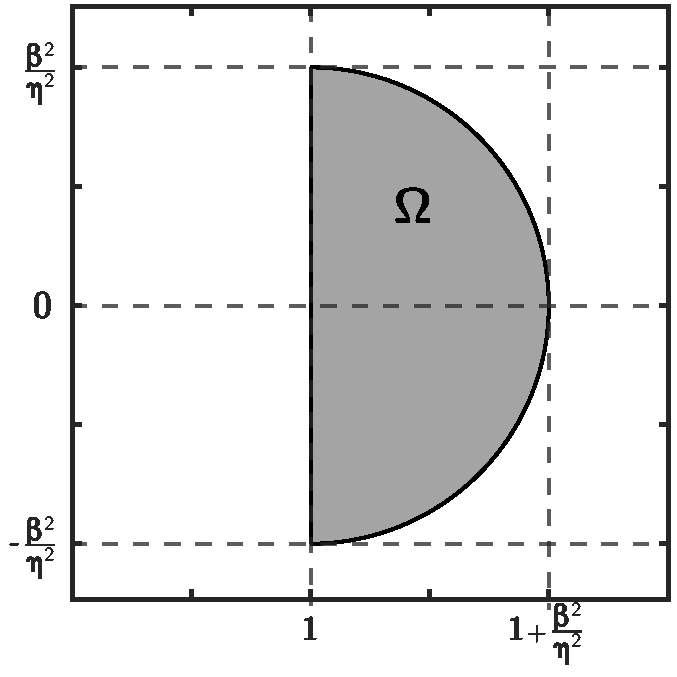
\includegraphics[width = 0.3\textwidth]{./figures/fov.pdf}
\caption{}
\label{fig:bound}
\end{figure}
\end{theorem}
\begin{proof}
Let $\sigma(B)$ denote the spectrum of operator $B$, $\sigma_{\textnormal{min}}(B)$
and $\sigma_{\textnormal{max}}(B)$ the minimum and maximum eigenvalues, and $\rho(B)$
the spectral radius. Also, define the symmetric/skew-symmetric splitting
$B = B_s + B_k$, where $B_s := (B+B^T)/2$ and $B_k := (B - B^T)/2$, and the numerical
radius as $r(B) = \sup \{ |\lambda| : \lambda \in W(B) \}$. Recall
the following properties of $W(B)$ \cite{gustafson1997numerical,mees1979domains}:
%
\begin{enumerate}
	\item $Bs \leq 0$ in the symmetric negative semi-definite sense
	if and only if $W(B) \leq 0$.  

	\item $W(B)\subset [\sigma_{\textnormal{min}}(B_s), \sigma_{\textnormal{max}}(B_s)] \times
	[-\rho(B_k)\mathrm{i}, \rho(B_k)\mathrm{i}]$.

	\item $\sigma(B) \subset W(B)$.

	% <Bv,v> + <v,Bv> > 0 ---> w = B^{-1}v ---> <w, B^{-1}w> + <B^{-1}w,w> > 0
	\item If $B$ is invertible and $B_s \leq 0$ in the symmetric negative semi-definite
	sense, then the symmetric part of $B^{-1}$ is also negative semi-definite.

	\item $r(B) \leq \|B\|_2$.

	\item $W(I + B) = 1 + W(B)$.
\end{enumerate}
%
Note that an exact inverse yields $\mathcal{P}_\eta = I$, with spectrum
and field-of-values given by $\sigma(\mathcal{P}_S) = W(\mathcal{P}_S) = \{1\}$.
Appealing to \eqref{eq:prec1} and the final property stated above, $W(\mathcal{P}_\eta)
= 1 + \tfrac{\beta^2}{\eta^2}W(E)$, for error term $E := (I - \tfrac{1}{\eta}\widehat{\mathcal{L}})^{-2}$
and real-valued constant $\beta^2/\eta^2 > 0$. Next we will bound $W(E)$ in the complex plane.

Assume that $\eta > 0$ and the symmetric part of $\widehat{\mathcal{L}}$ satisfies
$(\widehat{\mathcal{L}}+\widehat{\mathcal{L}}^T)/2 \leq 0$.
It follows that the real part of eigenvalues of $\widehat{\mathcal{L}}$ are non-positive and,
thus, $(I - \tfrac{1}{\eta}\widehat{\mathcal{L}})$ cannot have a zero eigenvalue and must be
invertible. Furthermore, it also follows that the symmetric part of
$(I - \tfrac{1}{\eta}\widehat{\mathcal{L}})$ is symmetric positive definite and thus
the symmetric part of $(I - \tfrac{1}{\eta}\widehat{\mathcal{L}})^{-2}$ is as well.
This yields a lower bound of zero on the real-axis for $W(E)$, that is,
Re$(W(E)) > 0$. 

Now, note that by the assumption $(\widehat{\mathcal{L}}+\widehat{\mathcal{L}}^T)/2 \leq 0$, we have
%
\begin{align}\label{eq:norm1}
\frac{\left\langle (I - \tfrac{1}{\eta}\widehat{\mathcal{L}})\mathbf{x},(I - \tfrac{1}{\eta}\widehat{\mathcal{L}})\mathbf{x}\right\rangle}
	{\langle\mathbf{x},\mathbf{x}\rangle} 
& = 1 - \frac{\langle (\widehat{\mathcal{L}} + \widehat{\mathcal{L}}^T )
	\mathbf{x},\mathbf{x}\rangle}{\eta \langle\mathbf{x},\mathbf{x}\rangle} +
	\frac{\langle \tfrac{1}{\eta^2}\widehat{\mathcal{L}}^T\widehat{\mathcal{L}}\mathbf{x},
	\mathbf{x}\rangle}{\langle\mathbf{x},\mathbf{x}\rangle}
\geq 1
\end{align}
%
for all $\mathbf{x}\neq\mathbf{0}$. Then,
%
\begin{align*}
\|(I - \tfrac{1}{\eta}\widehat{\mathcal{L}})^{-2}\| \leq \|(I - \tfrac{1}{\eta}\widehat{\mathcal{L}})^{-1}\|^2
& = \sup_{\mathbf{x}\neq\mathbf{0}} 
	\frac{\left\langle (I - \tfrac{1}{\eta}\widehat{\mathcal{L}})^{-1}\mathbf{x},
	(I - \tfrac{1}{\eta}\widehat{\mathcal{L}})^{-1}\mathbf{x}\right\rangle}
	{\langle\mathbf{x},\mathbf{x}\rangle} \\
&\hspace{-10ex}= \sup_{\mathbf{y}\neq\mathbf{0}} 
	\frac{\langle\mathbf{y},\mathbf{y}\rangle}{\left\langle (I - \tfrac{1}{\eta}\widehat{\mathcal{L}})\mathbf{y},
	(I - \tfrac{1}{\eta}\widehat{\mathcal{L}})\mathbf{y}\right\rangle}
\leq 1.
\end{align*}
%
This yields a bound on the numerical radius $r(E) = r((I - \tfrac{1}{\eta}\widehat{\mathcal{L}})^{-2})
\leq \|(I - \tfrac{1}{\eta}\widehat{\mathcal{L}})^{-2}\|\leq 1$. Combining with Re$(W(E)) > 0$,
the field of values of the error term, $W(E)$, is contained in the positive half of the
unit circle in the complex plane, which completes the proof.
\end{proof}
%

%
\begin{corollary}[GMRES convergence bounds]\label{cor:gmres}
Let $\pi_k$ denote the set of consistent polynomials of degree $k$. Then the ideal GMRES bound
(an upper bound in operator norm of worst-case convergence) on convergence after $k$ iterations
applied to the preconditioned operator $\mathcal{P}_\eta$ \eqref{eq:prec1} is bounded by
\begin{align*}
\min_{p\in\pi_k} \|p(\mathcal{P}_\eta)\| \leq 2\left(\frac{\beta^2/\eta^2}{2 + \beta^2/\eta^2}\right)^k.
\end{align*}
\end{corollary}
\begin{proof}
For operator $B$, let $\nu(B)$ denote the distance of $W(B)$ from the origin and define
$\cos(\zeta) := \nu(B) / r(B)$. In \cite[Lemma 3.2]{liesen2012field}, it is proven that worst-case convergence of GMRES applied to operator $B$ is bounded by
%
\begin{align}\label{eq:gmres}
\min_{p\in\pi_k} \|p(B)\| \leq 2\left(\frac{1-\cos\zeta}{1+\cos\zeta}\right)^k.
\end{align}
%
For $B = \mathcal{P}_\eta$, we have $\nu(\mathcal{P}_\eta)= 1$ and $r(\mathcal{P}_\eta) \leq 1+\beta^2/\eta^2$.
Plugging into \eqref{eq:gmres} completes the proof.\footnote{Note, classical GMRES convergence
results based on $\lambda_{\textnormal{min}}((\mathcal{P}_\eta+\mathcal{P}_\eta^T)/2)$ and
$\lambda_{\textnormal{max}}(\mathcal{P}_\eta^T\mathcal{P}_\eta)$ can also be applied, yielding
the bound $\Big(\tfrac{\beta^2/\eta^2}{1 + \beta^2/\eta^2}\Big)^{k/2}$, $2-4\times$
slower convergence than \Cref{th:fov}.}
\end{proof}
%

%
\begin{corollary}[CG convergence bounds]\label{cor:cg}
Define $\mathcal{Q}_\eta$ as in \eqref{eq:imag1} and $\mathcal{P}_\eta$ as in \eqref{eq:prec1},
and assume $(\eta I - \widehat{\mathcal{L}})$ is SPD. Then, the error $\mathbf{e}_k$ in the
$\mathcal{Q}_\eta$-norm after $k$ iterations of preconditioned conjugate gradient is bounded by
\begin{align*}
\frac{\|\mathbf{e}_k\|_{\mathcal{Q}_\eta}}{\|\mathbf{e}_0\|_{\mathcal{Q}_\eta}}
	\leq 2\left(\frac{\sqrt{1+\beta^2/\eta^2}-1}{\sqrt{1+\beta^2/\eta^2}+1}\right)^{k}.
\end{align*}
\end{corollary}
\begin{proof}
Note that if $(\eta I - \widehat{\mathcal{L}})$ is SPD, then $\mathcal{Q}_\eta$ is also
SPD. Then, recall that for conjugate gradient applied to SPD matrix $A$, error is
bounded via
\begin{align}\label{eq:cg_th}
\frac{\|\mathbf{e}_k\|_{A}}{\|\mathbf{e}_0\|_{A}}
	\leq 2\left(\frac{\sqrt{\kappa(A)}-1}{\sqrt{\kappa(A)}+1}\right)^{k},
\end{align}
where $\kappa(A)$ denotes the condition number of $A$. For preconditioned CG with 
SPD preconditioner $B^{-1}$ and Cholesky decomposition $B = R^TR$, PCG applied to
$A\mathbf{x}=\mathbf{b}$ is equivalent to applying CG to the modified SPD system
$(R^{-T}AR^{-1})R\mathbf{x} = R^{-T}\mathbf{b}$. The condition number is then given by
%
\begin{align*}
\kappa(R^{-T}AR^{-1}) & = \lambda_{max}(R^{-T}AR^{-1})/\lambda_{min}(R^{-T}AR^{-1}) \\
&= \lambda_{max}(R^{-1}R^{-T}A)/\lambda_{min}(R^{-1}R^{-T}A) \\
&= \lambda_{max}(B^{-1}A)/\lambda_{min}(B^{-1}A).
\end{align*}
%
for largest and smallest eigenvalues $\lambda_{max}$ and $\lambda_{min}$, respectively.
Then, recall that eigenvalues of an operator are contained in the field-of-values, and
from \Cref{th:fov}. This yields $\lambda_{max}(\mathcal{P}_\eta)/\lambda_{min}(\mathcal{P}_\eta)
\leq 1+\beta^2/\eta^2$, and by monotonicity of \eqref{eq:cg_th} in $\kappa$ this completes
the proof. 
% \begin{align*}
% \frac{\|\mathbf{e}_k\|_{\mathcal{Q}_\eta}}{\|\mathbf{e}_0\|_{\mathcal{Q}_\eta}}
% 	\leq 2\left(\frac{\sqrt{1+\beta^2/\eta^2}-1}{\sqrt{1+\beta^2/\eta^2}+1}\right)^{k}.
% \end{align*}
\end{proof}
%

\Cref{tab:beta} provides the values of $\eta$, $\beta^2/\eta^2$, and the CG and GMRES
bounds from \Cref{cor:gmres} and \Cref{cor:cg} for Gauss, RadauIIA, and LobattoIIIC
integration.

%
{
\renewcommand{\tabcolsep}{4pt}
\renewcommand{\arraystretch}{1.15}
\begin{table}[!ht]
  \centering
  \begin{tabular}{| c | c | c | cc | cc | ccc |}  % chktex 44
  \hline
& Stages & 2 & \multicolumn{2}{c}{3} & \multicolumn{2}{|c}{4} & \multicolumn{3}{|c|}{5} \\\hline\hline
\multirow{ 3}{*}{Gauss}
&$\eta$ & 3.0 & 4.64 & 3.68 & 4.21 & 5.79 & 7.29 & 4.65 & 6.70 \\
&$\beta^2/\eta^2$ & 0.33 & 0 & 0.91 & 1.59 & 0.09 & 0 & 2.36 & 0.27 \\
&CG & 0.072 & 0 & 0.160 & 0.234 & 0.022 & 0 & 0.294 & 0.060 \\
&GMRES & 0.143 & 0 & 0.313 & 0.444 & 0.043 & 0 & 0.541 & 0.119  \\\hline
\multirow{ 3}{*}{RadauIIA}
&$\eta$ & 2.0 & 3.64 & 2.68 & 3.21 & 4.79 & 6.29 & 3.66 & 5.70 \\
&$\beta^2/\eta^2$ & 0.50 & 0 & 1.29 & 2.21 & 0.11 & 0 & 3.20 & 0.32	\\
&CG & 0.101 & 0 & 0.205 & 0.283 & 0.025 & 0 & 0.344 & 0.069 \\
&GMRES & 0.2 & 0 & 0.393 & 0.525 & 0.051 & 0 & 0.616 & 0.137 \\\hline
\multirow{ 3}{*}{LobattoIIIC}
&$\eta$ & 1.0 & 2.63 & 1.69 & 2.22 & 3.78 & 5.28 & 2.66 & 4.70 \\
&$\beta^2/\eta^2$ & 1 & 0 & 2.21 & 3.51 & 0.13 & 0 & 4.88 & 0.38 \\
&CG & 0.172 & 0 & 0.284 & 0.360 & 0.031 & 0 & 0.416 & 0.081 \\
&GMRES & 0.333 & 0 & 0.525 & 0.637 & 0.063 & 0 &  0.709 & 0.161 \\
  \hline
  \end{tabular}
  \caption{$\eta$, $\beta^2/\eta^2$, and the convergence factors in \Cref{cor:gmres}
  and \Cref{cor:cg} for GMRES and CG, respectively (without the leading constants of
  2) for Gauss, RadauIIA, and LobattoIIIC integration,
  with 2--5 stages. Each column within a given set of stage columns corresponds to a
  single eigenvalue of $A_0^{-1}$. For odd numbers of stages, one eigenvalue is real,
  corresponding to the column where $\beta^2/\eta^2 = 0/\eta^2 = 0$.}\label{tab:beta}
\end{table}
% Gauss
% 2: 1.732050807568877^2/3.000000000000000^2
% 3: 0, 3.508761919567443^2/3.677814645373916^2			(4.644370709252176)
% 4: 5.31483608371350543^2/4.20757879435925566^2, 1.73446825786900750^2/5.79242120564074434^2
% 5: 0, 7.14204584067595280^2/4.64934860636329045^2, 3.48532283236639545^2/6.70391279830706629^2, 		(7.29347719065928652) 
% RadauIIA
% 2: 1.414213562373095^2/2^2
% 3: 0, 3.050430199247409^2/2.681082873627745^2	(3.637834252744503)
% 4: 4.77308743327664250^2/3.21280689687153398^2, 1.56747641689520812^2/4.78719310312846602^2
% 5: 0, 6.54373689936007729^2/3.65569432546357226^2, 3.21026560030854989^2/5.70095329867178942^2				(6.28670475172927665)
% Lobatto
% 2: 1
% 3: 0, 2.50873175492488^2/1.687091590520768^2 			(2.625816818958466)
% 4: 4.160391445506932^2/2.220980032989805^2, 1.38017652427285^2/3.779019967010193^2
% 5:
}

% ------------------------------------------------------------------------------------- %
\subsection{Conditioning independent of $\eta$ and $\beta$}\label{sec:solve:gamma}

In the previous section, we considered two applications of $(\eta I -
\widehat{\mathcal{L}})^{-1}$ as a preconditioner for $\mathcal{Q}_\eta$ \eqref{eq:imag1}.
\Cref{th:fov} and the corresponding Corollaries proved that preconditioned
GMRES is guaranteed to converge using such an approach, with bounds on convergence
provided in \Cref{tab:beta}. However, one can note from \Cref{fig:bound} and
\Cref{tab:beta} that convergence depends on values of $\beta$ and $\eta$ and, in
particular, that convergence degrades as the number of stages increase. Ideally,
we would like to observe convergence independent of $\beta$ and $\eta$, analogous
to spatial solvers that achieve convergence independent of spatial mesh and
discretization order. This section is motivated by \cite{exh}, where a similar
algorithm is developed for linear parabolic problems using the real Schur
decomposition, and, for SPD operators, a modified constant $\eta \mapsto
\sqrt{\eta^2+\beta^2}$ is proven to be optimal in terms of minimizing the
condition number of the preconditioned operator. In this section, we derive
bounds on the condition number of the preconditioned operator for
preconditioner $(\gamma I - \widehat{\mathcal{L}})^{-2}$, $\gamma\neq \eta$,
and general operators satisfying \Cref{ass:fov} (\Cref{th:cond}). A corollary
then proves that the constant 
%
\begin{align}\label{eq:gam_opt} 
\gamma _* := \sqrt{\eta^2+\beta^2}
\end{align}
%
yields a preconditioned operator with condition number $<9$, independent
of $\eta$ and $\beta$ (\Cref{cor:independent}).

Consider a similar preconditioner as in
\Cref{sec:solve:inv}, but with some modified constant $\gamma \mapsto
(\gamma I - \widehat{\mathcal{L}})^{-2}$. The resulting preconditioned
operator takes the form
%
\begin{align}\nonumber
\mathcal{P}_\gamma & = 
(\gamma I - \mathcal{L})^{-2}\Big[(nI - \mathcal{L})^2 + \beta^2 I\Big] \\ \nonumber
& = (\gamma I - \mathcal{L})^{-2}\Big[((\eta-\gamma)I + (\gamma I - \mathcal{L}))^2 + \beta^2 I\Big] \\
& = (\gamma I - \mathcal{L})^{-2}\Big[(\gamma-\eta)^2I - 2(\gamma-\eta)(\gamma I - \mathcal{L}) +
	(\gamma I - \mathcal{L})^2 + \beta^2 I\Big] \nonumber\\
& = I - 2(\gamma-\eta)(\gamma I - \mathcal{L})^{-1} + (\beta^2 + (\gamma-\eta)^2)(\gamma I - 
	\mathcal{L})^{-2} \nonumber\\
& = I - 2\frac{\gamma-\eta}{\gamma}\left(I - \tfrac{1}{\gamma}\mathcal{L}\right)^{-1} +
	\frac{\beta^2 + (\gamma-\eta)^2}{\gamma^2}
	\left(I - \tfrac{1}{\gamma}\mathcal{L}\right)^{-2}.\label{eq:prec_k}
\end{align}
%
Note that in \eqref{eq:prec_k} we have a quadratic polynomial in
$(I - \tfrac{1}{\gamma}\mathcal{L})^{-1}$. Although this provides
nice structure, the field-of-values analysis applied in \Cref{sec:solve:inv}
becomes much more complicated due to no necessary relation between
$\langle A\mathbf{x},\mathbf{x}\rangle$ and 
$\langle A^2\mathbf{x},\mathbf{x}\rangle$ for general operators $A$. Thus, here
we take a different approach, analyzing the condition number of the preconditioned
operator, $\mathcal{P}_\gamma$, similar to as done for SPD matrices in \cite{exh}.
Although the conditioning does not yield immediate GMRES bounds as the field-of-values
analysis does (or as conditioning does for bounds on CG convergence), it still
provides a robust measure of the effectiveness and scalability of the 
preconditioner.

As a preliminary result, note that working out the roots of the polynomial 
in \eqref{eq:prec_k}, it can be expressed in factored form as
%
\begin{align*}
\mathcal{P}_\gamma
	& = \Big[I - \overline{\alpha}\left(I - \tfrac{1}{\gamma}\mathcal{L}\right)^{-1}\Big]
	\Big[I - \alpha\left(I - \tfrac{1}{\gamma}\mathcal{L}\right)^{-1}\Big],
\end{align*}
%
where
%
\begin{align}\label{eq:alpha}
\alpha, \overline{\alpha} & := 1 - \frac{\eta}{\gamma} \pm \mathrm{i}\beta,
\end{align}
%
and
%
\begin{align}\label{eq:alpha_eq}
\alpha + \overline{\alpha} = 2(1 - \tfrac{\eta}{\gamma}), \hspace{5ex}
\alpha\overline{\alpha} = \tfrac{\beta^2 + (\gamma-\eta)^2}{\gamma^2}.
\end{align}
%
Moving forward we will limit ourselves to considering $\eta \leq \gamma \leq \
\tfrac{\eta^2+\beta^2}{\eta}$, which limits to the natural case of $\gamma = \eta$
as $\beta \to 0$. Similar analysis can be performed for $\gamma$ outside of
this range, but the derivations are different and there does not appear to
be any good reason for $\gamma$ outside of this range (see discussion
following \Cref{th:cond}).

%
\begin{theorem}[Conditioning of preconditioned operator]\label{th:cond}
Suppose Assumptions \ref{ass:eig} and \ref{ass:fov} hold, that is, $\eta > 0$
and $W(\mathcal{L}) \leq 0$ \eqref{eq:fov}. Let $\eta \leq \gamma \leq \
\tfrac{\eta^2+\beta^2}{\eta}$ and let
$\mathcal{P}_\gamma$ denote the preconditioned operator, where $((\eta + i\beta)I -
\widehat{\mathcal{L}})((\eta - i\beta)I - \widehat{\mathcal{L}})$ is
preconditioned with $(\gamma I - \widehat{\mathcal{L}})^{-2}$. Then,
\begin{align}\label{eq:cond1}
\textnormal{cond}(\mathcal{P}_\gamma) \leq (1 + \alpha\overline{\alpha})
		\left(1 + \frac{\alpha\overline{\alpha}}{(1 - \alpha)(1 - \overline{\alpha})}\right)
	% \begin{cases} 
	% \frac{1 + \alpha\overline{\alpha}} {(1 - \alpha)(1 - \overline{\alpha})}
	% 	& \eta\gamma \geq \eta^2+\beta^2, \\
	% (1 + \alpha\overline{\alpha})
	% 	\left(1 + \frac{\alpha\overline{\alpha}}{(1 - \alpha)(1 - \overline{\alpha})}\right)
	% 	& \eta\gamma < \eta^2+\beta^2,
	% \end{cases}
\end{align}
with $\alpha$ and $\overline{\alpha}$ defined as in \eqref{eq:alpha}.
\end{theorem}
\begin{proof}
The proof proceeds as follows: first, we factor $\mathcal{P}_\gamma$ \eqref{eq:prec_k},
and proceed to use the factored form to derive an upper bound on 
$\|\mathcal{P}_\gamma\|$ and $\|\mathcal{P}_\gamma^{-1}\|$, which immediately
yields a bound on
%
\begin{align}\label{eq:cond0}
\textnormal{cond}(\mathcal{P}_\gamma) = \|\mathcal{P}_\gamma\|\|\mathcal{P}_\gamma^{-1}\|.
\end{align}
%
Note that following from the discussion in \Cref{sec:solve:inv} and \Cref{th:fov},
for real $k>0$, $W\left[\left(I - \tfrac{1}{k}\mathcal{L}\right)^{-1}\right]$ and
$W\left[\left(I - \tfrac{1}{k}\mathcal{L}\right)^{-2}\right]$ are contained in
the positive half unit circle, and $\|(I - \tfrac{1}{\gamma}\mathcal{L})^{-1}\| \leq 1$
(see proof of \Cref{th:fov}).

We start with $\|\mathcal{P}_\gamma\|$, where
%
\begin{align}\label{eq:CS}
\|\mathcal{P}_\gamma\| & \leq 
	\Big\|I - \overline{\alpha}\left(I - \tfrac{1}{\gamma}\mathcal{L}\right)^{-1}\Big\|
	\Big\|I - \alpha\left(I - \tfrac{1}{\gamma}\mathcal{L}\right)^{-1}\Big\|.
\end{align}
%
Recalling that $W\left[(I - \tfrac{1}{k}\mathcal{L})^{-1}\right] \geq 0$
and $\|(I - \tfrac{1}{\gamma}\mathcal{L})^{-1}\| \leq 1$, and using the
assumption $\gamma \geq \eta$, we can expand the norm squared in inner-product
form, yielding
%
\begin{align*}
&\hspace{-5ex}
\Big\|I - \overline{\alpha}\left(I - \tfrac{1}{\gamma}\mathcal{L}\right)^{-1}\Big\|^2 \\
	& = 1 + \max_{\mathbf{x}\neq\mathbf{0}} \left( \alpha\overline{\alpha}
		\frac{\left\|\left(I - \tfrac{1}{\gamma}\mathcal{L}\right)^{-1}\mathbf{x}\right\|^2
		}{\|\mathbf{x}\|^2}
	- (\alpha + \overline{\alpha})\frac{\textnormal{Re}\left(\left\langle\left(I -
		\tfrac{1}{\gamma}\mathcal{L}\right)^{-1}\mathbf{x}, \mathbf{x}\right\rangle\right)}
		{\|\mathbf{x}\|^2}\right) \\
& \leq 1 + \alpha\overline{\alpha}\left\|\left(I - \tfrac{1}{\gamma}\mathcal{L}\right)^{-1}\right\|^2 \\
& \leq 1 + \alpha\overline{\alpha}.
\end{align*}
%
Note that the above derivation is identical for $\alpha$ and $\overline{\alpha}$,
which yields
%
\begin{align} \label{eq:upper_alpha}
\|\mathcal{P}_\gamma\| & \leq 1 + \alpha\overline{\alpha}.
\end{align}
%

To bound $\|\mathcal{P}_\gamma^{-1}\|$, we use an analogous approach as above
\eqref{eq:CS}, developing bounds on the two polynomial factors separately.
First, note that
%
\begin{align}\nonumber
\left[I - \alpha\left(I - \tfrac{1}{\gamma}\mathcal{L}\right)^{-1}\right]^{-1}
	& = \left(I - \tfrac{1}{\gamma}\mathcal{L}\right)
		\left[(1-\alpha)I - \tfrac{1}{\gamma}\mathcal{L}\right]^{-1} \nonumber\\
& = \left[\alpha I + ((1-\alpha)I - \tfrac{1}{\gamma}\mathcal{L})\right]
		\left[(1-\alpha)I - \tfrac{1}{\gamma}\mathcal{L}\right]^{-1} \nonumber\\
& = I + \alpha \left[(1-\alpha)I - \tfrac{1}{\gamma}\mathcal{L}\right]^{-1} \nonumber\\
& = I + \frac{\alpha}{1-\alpha} \left(I - \tfrac{1}{\gamma(1-\alpha)}\mathcal{L}\right)^{-1}.
	\label{eq:inv_factor}
\end{align}
%
For condensed notation, let $c_\alpha := \tfrac{\alpha}{1-\alpha}$, and note that 
%
\begin{align*} 
c_\alpha+\overline{c_\alpha} & = \frac{\alpha + \overline{\alpha} - 2\alpha\overline{\alpha}}
	{1 + \alpha\overline{\alpha} - (\alpha + \overline{\alpha})} 
= \frac{2\eta\gamma - 2(\eta^2+\beta^2)}{\eta^2+\beta^2},
\end{align*}
%
which is $< 0$ when $\eta\gamma \leq (\eta^2+\beta^2)$ and $<0$ otherwise. 

Expanding the squared norm of \eqref{eq:inv_factor} in inner-product form, we have
%
\begin{align}\label{eq:pinv0}
& \hspace{-5ex}
1 + \max_{\mathbf{x}\neq\mathbf{0}} \left[ (c_\alpha+\overline{c_\alpha})
	\frac{\textnormal{Re}\left(\left\langle (I - \tfrac{1}{\gamma(1-\alpha)}\mathcal{L})^{-1}\mathbf{x},
		\mathbf{x}\right\rangle\right)}{\|\mathbf{x}\|^2} + 
	c_\alpha\overline{c_\alpha}
	\frac{\left\|(I - \tfrac{1}{\gamma(1-\alpha)}\mathcal{L})^{-1}\mathbf{x}\right\|^2}
		{\|\mathbf{x}\|^2} \right].
\end{align}
%
Bounding the norm term in \eqref{eq:pinv0} requires care because $\alpha$ is
complex. Note that the norm is the maximum singular value, which is equivalent to one
over the minimum nonzero singular value of the inverse. The squared minimum nonzero
singular value of the inverse of the inverse is given by
%
\begin{align*}
&\hspace{-5ex}
\min_{\mathbf{x}\neq\mathbf{0}} \frac{\left\|\left(I - \tfrac{1}{\gamma(1-\alpha)}
	\mathcal{L}\right)\mathbf{x}\right\|^2}{\|\mathbf{x}\|^2} \\
& = 1 + \min_{\mathbf{x}\neq\mathbf{0}} \left[ \frac{1}{|\gamma(1-\alpha)|^2}
	\frac{\left\|\mathcal{L}\mathbf{x}\right\|^2}{\|\mathbf{x}\|^2}
	- \left(\frac{1}{\gamma(1-\alpha)} + \frac{1}{\overline{\gamma}(1-\overline{\alpha})}\right)
	\frac{\textnormal{Re}\left(\left\langle\mathcal{L}\mathbf{x},\mathbf{x}\right\rangle\right)}
		{\|\mathbf{x}\|^2}\right].
\end{align*}
%
Noting that Re$\left(\langle\mathcal{L}\mathbf{x},\mathbf{x}\rangle\right) \leq 0$,
$\gamma \geq \eta > 0$, and Re$(1-\alpha) \geq 0$, it follows that the squared minimum
singular value above is $\geq 1$, which implies $\|(I - \tfrac{1}{\gamma(1-\alpha)}
\mathcal{L})^{-1}\| \leq 1$.

% ------> Old extra derivation for \gamma larger than currently considered
% ------------------------------------------------------------------------
% Plugging into \eqref{eq:pinv1} and noting
% that an identical derivation and result holds for $\overline{\alpha}$, we have
% for $(c_\alpha+\overline{c_\alpha}) \geq 0$,
% %
% \begin{align}\nonumber
% \|\mathcal{P}_\gamma^{-1}\| & \leq 
% 	\Big\|\Big(I - \overline{\alpha}\left(I - \tfrac{1}{\gamma}\mathcal{L}\right)^{-1}\Big)^{-1}\Big\|
% 	\Big\|\Big(I - \alpha\left(I - \tfrac{1}{\gamma}\mathcal{L}\right)^{-1}\Big)^{-1}\Big\| \\
% & \leq \left(1 + \frac{\alpha}{1-\alpha}\right)
% 	\left(1 + \frac{\overline{\alpha}}{1-\overline{\alpha}}\right) \nonumber\\
% & = \frac{1}{(1 - \alpha)(1 - \overline{\alpha})}. \label{eq:lower_alpha1}
% \end{align}
% %

Returning to \eqref{eq:pinv0}, consider the inner-product term with leading
constant $(c_\alpha+\overline{c_\alpha}) \leq 0$. Note that letting
$\mathbf{x}:= (I - \tfrac{1}{\gamma(1-\alpha)}\mathcal{L})\mathbf{y}$,
we have
%
\begin{align*}
\frac{\left\langle (I - \tfrac{1}{\gamma(1-\alpha)}\mathcal{L})^{-1}\mathbf{x},
		\mathbf{x}\right\rangle}{\|\mathbf{x}\|^2}
& = \frac{\left\langle \mathbf{y}, (I - \tfrac{1}{\gamma(1-\alpha)}\mathcal{L})\mathbf{y}
	\right\rangle}{\|(I - \tfrac{1}{\gamma(1-\alpha)}\mathcal{L})\mathbf{y}\|^2}
= \frac{\|\mathbf{y}\|^2 - \frac{1}{\gamma (1 - \overline{\alpha})}
	\left\langle \mathbf{y},\mathcal{L}\mathbf{y} \right\rangle}
	{\|(I - \tfrac{1}{\gamma(1-\alpha)}\mathcal{L})\mathbf{y}\|^2}.
\end{align*}
%
By assumption, Re$\left(\langle \mathbf{y},\mathcal{L}\mathbf{y}\rangle\right) \leq 0$,
while $\gamma\geq 0$ and Re$(1-\alpha) \geq 0$. It follows that
%
\begin{align*}
\textnormal{Re}\left(\frac{\left\langle (I - \tfrac{1}{\gamma(1-\alpha)}\mathcal{L})^{-1}\mathbf{x},
	\mathbf{x}\right\rangle}{\|\mathbf{x}\|^2}\right) \geq 0.
\end{align*}
%
Thus in \eqref{eq:pinv0} because $(c_\alpha+\overline{c_\alpha}) \leq 0$, we can drop
the corresponding term for an upper bound of
%
\begin{align*}
\left\|\left[I - \alpha\left(I - \tfrac{1}{\gamma}\mathcal{L}\right)^{-1}\right]^{-1}\right\|^2 
	& \leq 1 + c_\alpha\overline{c_\alpha}
		\left\|(I - \tfrac{1}{\gamma(1-\alpha)}\mathcal{L})^{-1}\right\|^2 \\
& \leq 1 + c_\alpha\overline{c_\alpha} \\
& = 1 + \frac{\alpha\overline{\alpha}}{(1 - \alpha)(1 - \overline{\alpha})}.
\end{align*}
%
Again noting that analogous derivations holds for $\overline{\alpha}$ with
identical bounds, we have for $(c_\alpha+\overline{c_\alpha}) < 0$,
%
\begin{align}
\|\mathcal{P}_\gamma^{-1}\| & \leq 1 + 
	\frac{\alpha\overline{\alpha}}{(1 - \alpha)(1 - \overline{\alpha})}. \label{eq:lower_alpha2}
\end{align}
% 

Combining \eqref{eq:cond0}, \eqref{eq:upper_alpha},
and \eqref{eq:lower_alpha2} completes the proof.
\end{proof}
%

In \cite{exh}, a similar analysis as \Cref{th:cond} is done under the assumption
that $-\mathcal{L}$ is SPD, in which case the conditioning can be derived based on
eigenvalues. There, they derive the (exact) conditioning of the preconditioned
operator for $\gamma = \eta$ to be cond$(\mathcal{P}_\eta) = 1 + \tfrac{\beta^2}{\eta^2}$.
If we let $\gamma = \eta$, from \eqref{eq:alpha_eq} we have
$\alpha+\overline{\alpha} = 0$, $\alpha\overline{\alpha} =
\frac{\beta^2}{\eta^2}$, and \Cref{th:cond} yields the bound
%
\begin{align}\label{eq:cond_eta}
\textnormal{cond}(\mathcal{P}_{\gamma = \eta}) \leq 1 + 2\frac{\beta^2}{\eta^2}.
\end{align}
%
In particular, this indicates that \Cref{th:cond} is fairly tight (it is unclear
if the additional factor of 2 in \eqref{eq:cond_eta} is necessary for non-SPD
operators, or a flaw in the line of proof). 
Considering the upper limit on $\gamma$ in \Cref{th:cond}, $\gamma \mapsto
\tfrac{\eta^2+\beta^2}{\eta}$, we have a bound
%
\begin{align}\label{eq:cond_upper}
\textnormal{cond}\left(\mathcal{P}_{\gamma = \frac{\eta^2+\beta^2}{\eta}}\right) \leq
	\left(1 + \frac{\beta^2}{\eta^2}\right) \left(1 + \frac{\beta^2}{\beta^2 + \eta^2}\right).
\end{align}
%
Note, in both \eqref{eq:cond_eta} and \eqref{eq:cond_upper} we see a dependence
on $\eta$ and $\beta$.

Using the tight derivation of conditioning of the preconditioned operator in
\cite{exh}, they also derive an optimal constant to minimize the condition
number for SPD matrices, $\gamma _* := \sqrt{\eta^2+\beta^2}$ \eqref{eq:gam_opt}.
Considering $\gamma_*$ here, \eqref{eq:alpha_eq} yields
$\alpha+\overline{\alpha} = \alpha\overline{\alpha} =
2 - 2\frac{\eta}{\sqrt{\eta^2+\beta^2}}$, and \Cref{th:cond} yields the bound
%
\begin{align}\label{eq:cond_opt}
\textnormal{cond}(\mathcal{P}_{\gamma_*})
	\leq \left(3 - 2\frac{\eta}{\sqrt{\eta^2+\beta^2}}\right)^2.
\end{align}
%
Noting that $\textnormal{cond}(\mathcal{P}_{\gamma_*}) < 9$ for all $\eta>0,
\beta\geq 0$, we have the following corollary.

%
\begin{corollary}[Conditioning independent of $\eta$ and $\beta$]\label{cor:independent}
Preconditioning $\mathcal{Q}_\eta$ \eqref{eq:imag1} with
$(\gamma_* I - \widehat{\mathcal{L}})^{-2}$, for $\gamma_* = \sqrt{\eta^2+\beta^2}$
yields a preconditioned operator $\mathcal{P}_{\gamma_*}$ such that
$\textnormal{cond}(\mathcal{P}_{\gamma_*}) < 9$,
independent of $\eta$ and $\beta$.
\end{corollary}
%
It is also worth pointing out that as $\beta \to 0$, $\gamma \to \eta$
in all three of the above cases, and (as expected) \eqref{eq:cond_eta},
\eqref{eq:cond_upper}, and \eqref{eq:cond_opt} all $\to 1$.

%
\begin{remark}[``Optimal'' $\gamma$]
A natural question is what is the optimal $\gamma$ in general?
Let $f(\gamma)$ denote the upper bound from \Cref{th:cond} \eqref{eq:cond1}.
Some algebra shows that
%
\begin{align*}
f'(\gamma) &= \frac{4\gamma^4 - 6\eta\gamma^3 + 4\eta(\eta^2+\beta^2)\gamma -
	2(\eta^2+\beta^2)^2}{(\eta^2+\beta^2)\gamma^3}.
\end{align*}
%
For $\beta > 0$,
%
\begin{align*}
f'(\eta) & = -\frac{2\beta^4}{\eta^3(\eta^2+\beta^2)} < 0, 
\hspace{5ex}
f'(\gamma_*) = \frac{2(\sqrt{\eta^2+\beta^2} - \eta)}{\eta^2+\beta^2} > 0.
% f'\left(\tfrac{\eta^2+\beta^2}{\eta}\right) & = 2\beta^2 + \frac{\beta^2}{\eta^2+\beta^2} > 0, \\
\end{align*}
%
Thus there exists a critical point $\gamma \in(\eta,\gamma_*)$, and it is 
likely not advantageous to choose $\gamma > \gamma_*$. The equation
for the root is a quartic polynomial and is not examined analytically here,
however, depending on $\eta$ and $\beta$, the sign change (and, thus, root) is
likely between $0.8\gamma_* - 0.9\gamma_*$ , suggesting $\gamma_*$ is indeed
a good approximation to the optimal $\gamma$ with respect to \eqref{eq:cond1}.

Moreover, the analysis from \cite{exh} proves that $\gamma_*$ \eqref{eq:gam_opt}
\textit{is} optimal for SPD operators, and we prove $\gamma_*$ also provides
very good preconditioning independent of the number of stages/order of integration
in the more general setting (\Cref{cor:independent}).
\end{remark}
%



% ------------------------------------------------------------------------------------- %
% ------------------------------------------------------------------------------------- %
\subsection{Preconditioning in practice}


% ------------------------------------------------------------------------------------- %
\subsubsection{Choosing $\gamma$}



% ------------------------------------------------------------------------------------- %
\subsubsection{Inexact preconditioning}

In practice, fully converging $(\eta I - \widehat{\mathcal{L}})^{-1}$ as a preconditioner
is not desirable --  even if a Krylov method converges rapidly, if each iteration requires
a full linear solve, the resulting method remains too expensive to be competitive in practice.
Here, we propose
applying a Krylov method to $\mathcal{Q}_\eta:=(\eta^2+\beta^2)I - 2\eta\widehat{\mathcal{L}} +
\widehat{\mathcal{L}}^2$ by computing the operator's action (that is, not fully constructing
it), and preconditioning each Krylov iteration with \textit{two} applications of a sparse
parallel preconditioner for $(\eta I - \widehat{\mathcal{L}})$, approximating the action
of $(\eta I - \widehat{\mathcal{L}})^{-2}$.

To motive this heuristically, suppose $(\eta I - \widehat{\mathcal{L}}) = B + N$,
where $B^{-1}$ corresponds to the action of a preconditioner and $N$ the error
term that is not captured. For a good preconditioner, we expect
$B^{-1}(\eta I - \widehat{\mathcal{L}}) = I+B^{-1}N$ to be
well-conditioned and, thus, $B^{-1}N$ to be small in some sense. Then,
%
\begin{align}\nonumber
B^{-2}\mathcal{Q}_\eta & = I + \beta^2B^{-2} + \left(B^{-2}NB + B^{-1}N + B^{-2}N^{-2}\right)\label{eq:approx}.
\end{align}
%
In addition to wanting $N$ to be small, it is also important that the error terms
$B^{-2}NB + B^{-1}N + B^{-2}N^{-2}$ are generally positive in a field-of-values sense.
If these terms are large and positive in a field-of-values sense, the outer Krylov
iteration applied to $B^{-2}\mathcal{Q}_\eta$ can correct for these modes. However,
if error terms $B^{-2}NB + B^{-1}N + B^{-2}N^{-2}$ in \eqref{eq:approx} have 
negative components, the field-of-values of the preconditioned operator is shifted
towards the origin, wherein Krylov acceleration is often of progressively less use. 

Thus, theory developed in \Cref{sec:solve:prec} guarantees that the proposed algorithm
will have robust and fairly rapid convergence under reasonable assumptions if each
linear system is inverted exactly. Approximate inverses prove to be much faster in
practice, but \textit{it is important that the underlying preconditioner provides a good
inverse approximation}. Fortunately, for difficult problems with only okay preconditioners,
it is straightforward to apply either multiple inner fixed-point iterations or an
inner Krylov iteration (wrapped with a flexible outer Krylov method
\cite{notay2000flexible,saad1993flexible}) to ensure robust (outer) iterations, analogous
to techniques used in block preconditioning. In \Cref{sec:numerics:dg:diff}, a
numerical example is shown where the proposed method diverges using a single inner
fixed-point iteration as a preconditioner for $(\eta I - \widehat{\mathcal{L}})$, but
three (or more) inner fixed-point iterations yields fast, scalable convergence.

% ------------------------------------------------------------------------------------- %
\subsubsection{Mass matrices}

Recall in the finite element context where mass matrices are involved, we defined
$\widehat{\mathcal{L}} := \delta t M^{-1}\mathcal{L}$. For a given conjugate pair
of eigenvalues, the quadratic polynomial \eqref{eq:imag1} can be expressed as
%
\begin{align}\label{eq:scaleM}
\mathcal{Q}_\eta = M^{-1}((\eta + i\beta)M - \delta t{\mathcal{L}})M^{-1}((\eta - i\beta)M -
	\delta t\widehat{\mathcal{L}}).
\end{align}
%
In this context, it is best to first scale both sides of the linear system by $M$.
This halves the number of times $M^{-1}$ must applied for each Krylov iteration,
and if $M$ and $\mathcal{L}$ are Hermitian, the resulting quadratic system is SPD
and can be solved using preconditioned conjugate gradient or MINRES, preconditioned
with one application of a preconditioner, the action of $M$, and a second application
of the preconditioner.


% ------------------------------------------------------------------------------------- %
% ------------------------------------------------------------------------------------- %
% ------------------------------------------------------------------------------------- %
\begin{comment}
\section{Implementation details:  The time-independent case}
The basic idea is that we need to do the update
\begin{align} \label{eq:RK_update}
\bm{u}_{n+1}  = \bm{u}_n + \delta t \mdet({\cal M}_s)^{-1} \big( \bm{b}_0^\top A^{-1}_0 \otimes I \big) \madj({\cal M}_s) \bm{f},
\end{align}
where we have
\begin{itemize}
\item $m \in \mathbb{N}$: The dimension of the spatial problem

\item $\bm{f} = (\bm{f}_1, \ldots, \bm{f}_s)^\top$, with $\bm{f}_j \in \mathbb{R}^m$

\item $\tilde{\bm{b}}^\top_0 \coloneqq \bm{b}^\top_0 A^{-1}_0 \in \mathbb{R}^{1 \times s}$ (this is a row vector, not that this distinction really matters) 
\end{itemize}

Now we break \eqref{eq:RK_update} into two steps:
\begin{enumerate}
\item{Step 1:}\label{it:update_step1}Compute 
\begin{align} \label{eq:step1}
\bm{z} = \big( \hat{\bm{b}}^\top_0 \otimes I \big) \madj ({\cal M}_s) \bm{f} \in \mathbb{R}^m
\end{align}

\item{Step 2:}\label{it:update_step2} Solve
\begin{align} \label{eq:step2}
\mdet( {\cal M}_s ) \bm{y} = \bm{z},
\end{align}
then update per \eqref{eq:RK_update}, $\bm{u}_{n+1} = \bm{u}_n + \delta t \bm{y}$
\end{enumerate}


\subsection{On Step \ref{it:update_step1}}

The adjugate of ${\cal M}_s$ is a matrix defined over degree  $s-1$ polynomials in ${\cal L} \in \mathbb{R}^{m \times m}$. More specifically, we write it as
\begin{align}
\madj ({\cal M}_s) = 
\begin{bmatrix}
Q_{11}({\cal L}) & \cdots & Q_{1s}({\cal L}) \\
\vdots & & \vdots \\
Q_{s1}({\cal L}) & \cdots & Q_{ss}({\cal L})
\end{bmatrix}
\in \mathbb{R}^{ms \times ms},
\quad
Q_{ij}({\cal L}) = \sum \limits_{k = 0}^{s-1} \hat{q}_{ijk} {\cal L}^k \in \mathbb{R}^{m \times m}.
\end{align}

Now, the Kronecker product appearing in front of this matrix simply takes inner products over its columns to give a block rectangular matrix whose elements are therefore polynomials in ${\cal L}$ of degree $s-1$:
\begin{align}
\big( \bm{b}_0^\top A^{-1}_0 \otimes I \big) \madj({\cal M}_s) 
=
\begin{bmatrix}
X_{1}({\cal L}), \, \cdots, \, X_{s}({\cal L})
\end{bmatrix},
\end{align}
where
\begin{align}
X_{j}({\cal L}) = \sum \limits_{k = 0}^{s-1} \hat{x}_{j k} {\cal L}^k \in \mathbb{R}^{m \times m}, 
\quad
\hat{x}_{j k} = \sum \limits_{\ell = 1}^s \big( \tilde{\bm{b}}_0^\top \big)_{\ell} \hat{q}_{\ell j k}.
\end{align}
And, so, finally, the vector in \eqref{eq:step1} can be written as the sum
\begin{align} \label{eq:z_sum}
\bm{z} = \sum \limits_{i = 1}^s X_i({\cal L}) \bm{f}_i.
\end{align}
The main task here is going to be computing the action of the degree $s-1$ polynomials $X_i({\cal L})$ of the components of $\bm{f}$; note that we can  easily compute the sets of coefficients $\{ x_{jk} \}_{(j,k)=(1,0)}^{(s,s-1)}$. I think the most efficient way to compute the action of this polynomial is with a Horner-like scheme which is a well-known technique for evaluating scalar polynomials (see \url{https://en.wikipedia.org/wiki/Horner\%27s_method}). Basically, we can compute the action of the $n$th degree polynomial $P_n({\cal L})$ on a vector using: $n$ \texttt{MATVECs} with ${\cal L}$, $n+1$ \texttt{AXPYs} ($\bm{x} \gets \alpha \bm{y} + \beta \bm{z}$), $n$ \texttt{copies} ($n$ lots of copying values from one vector to another, $n \times [\bm{x} \gets \bm{y}]$), and one intermediate/temporary vector. So the main cost in computing \eqref{eq:z_sum} is $s(s-1)$ \texttt{MATVECs} with ${\cal L}$.
\end{comment}

% ------------------------------------------------------------------------------------- %
% ------------------------------------------------------------------------------------- %
% ------------------------------------------------------------------------------------- %
\section{Numerical results}\label{sec:numerics}

% ------------------------------------------------------------------------------------- %
% ------------------------------------------------------------------------------------- %
\subsection{Finite-difference advection-diffusion}\label{sec:numerics:fd}
\todo{Is it relevant that I ran these tests on my laptop using 4 procs; is this something that should be added in?}

In this section, we consider a constant-coefficient advection-diffusion problem discretized in space with high-order finite-differences. An exact solution to this problem is used to demonstrate the high-order accuracy of the IRK methods, and the robustness of the algorithms developed in the previous section with respect to mesh resolution. Specifically, we solve the PDE
\begin{align} \label{eq:FD_ex}
u_t + 0.85 u_x + u_y = 0.3 u_{xx} + 0.25 u_{yy} + s(x,y,t),
\quad (x,y,t) \in (-1,1)^2 \times (0,2],
\end{align}
on a periodic spatial domain. The source term $s(x,y,t)$ is chosen such that the solution of the PDE is $u(x,y,t)=\sin^4(\pi/2[x-1-0.85t]) \sin^4(\pi/2 [y-1-t]) \exp(-[0.3+0.25]t)$. 

We consider tests using IRK methods of orders three, four, seven, and eight. The 3rd- and 4th-order IRK methods are paired with 4th-order central-finite-differences in space, and the 7th- and 8th-order methods with 8th-order central-finite-differences in space. In all cases, a time-step of $\delta t = 2 h$ is used, with $h$ denoting the spatial mesh size. Due to the non-SPD nature of the spatial discretization, we apply GMRES(30) as the linear solver, for which absolute and relative stopping tolerances of $10^{-13}$ are employed. To precondition solves involving matrices of the form $\gamma_* I - \delta t {\cal L}$, a single iteration of \textit{hypre}'s Boomer AMG (interfaced through \textit{mfem}) is used. Boomer AMG is employed with classical interpolation (type 0), Falgout coarsening (type 6) with a strength tolerance $\theta_C = 0.25$ and zero levels of aggressive coarsening, and $L_1$-Gauss--Seidel relaxation (type 8). 

In Fig. \ref{fig:FD_ex}, discretization errors are shown for these test problems, alongside the average number of AMG iterations needed per time step. The expected asymptotic convergence rates are observed for all discretizations\footnote{An exception here is A--SDIRK(4), which appears to be converging with a rate closer to three than four; however, further decreasing $\delta t$ (not shown here) confirms 4th-order convergence is achieved eventually.} since the curves have the same slopes as the black, dashed reference lines with slopes three, four, seven, and eight shown in the left panel of the figure. 

The preconditioner appears robust with respect to mesh and problem size, since the average number of AMG iterations per time step (which is a proxy for the number of GMRES iterations) remains roughly constant as the the mesh is refined.
%
Of the fully implicit methods, Gauss appears to be the most efficient since it requires the fewest AMG iterations. The Gauss methods are closely followed by the Radau IIA methods, with the Lobatto IIC methods somewhat slower. This is consistent with the earlier described theoretical results (see Table \ref{tab:beta}). Note that while Gauss and Radau IIA methods have very similar iteration counts, Gauss converges at one order faster, which can be seen in the left-hand panel of the figure.
%
Considering the lower-order methods in the top row of Fig. \ref{fig:FD_ex}, L--SDIRK(4), a 5-stage, 4th-order, L-stable SDIRK method requires the most AMG iterations of all methods. A--SDIRK(4), a 3-stage, 4th-order, A-stable SDIRK method, requires far fewer AMG iterations than L--SDIRK(4).  However, A--SDIRK(4) yields a significantly larger discretization error than the other 4th-order schemes, and takes longer to reach its asymptotic convergence rate. Thus, in terms of work done per accuracy, A--SDIRK(4) is certainly not competitive with Gauss(4) for this particular test problem.

\begin{figure}[!htb]
%\begin{figure}[H]
\centerline{
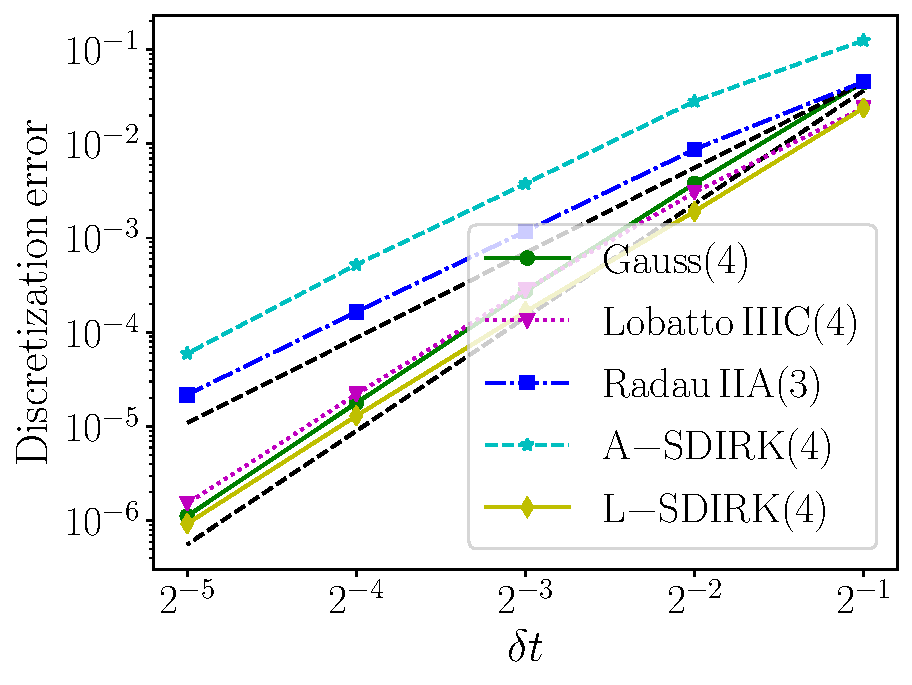
\includegraphics[width = 0.475\textwidth]{figures/FD_ex/errors_iters_14_34_23_-14_4_d2_ex1.pdf}
\quad
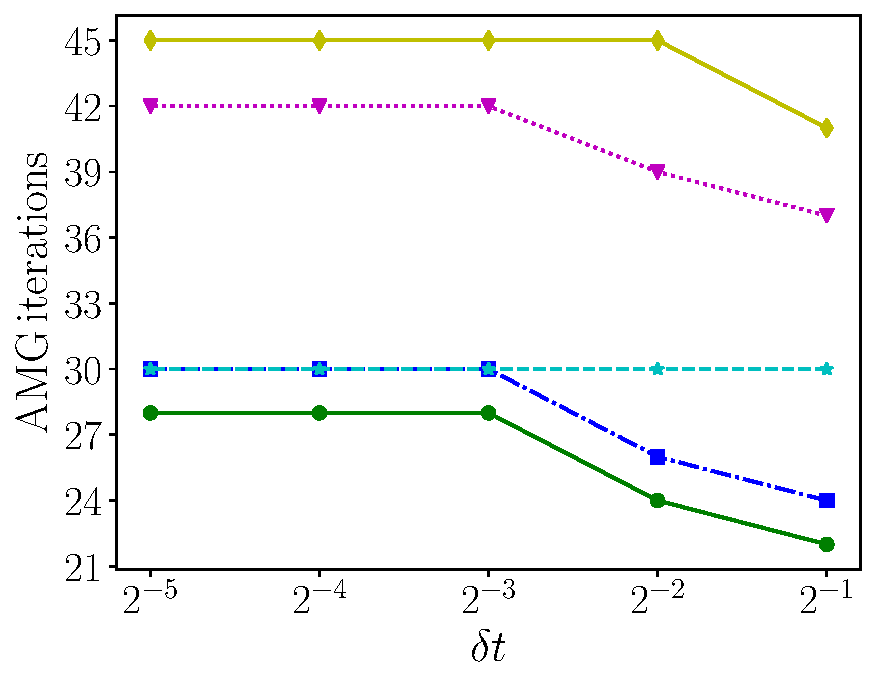
\includegraphics[width = 0.475\textwidth]{figures/FD_ex/amg_iters_14_34_23_-14_4_d2_ex1.pdf}
}
\centerline{
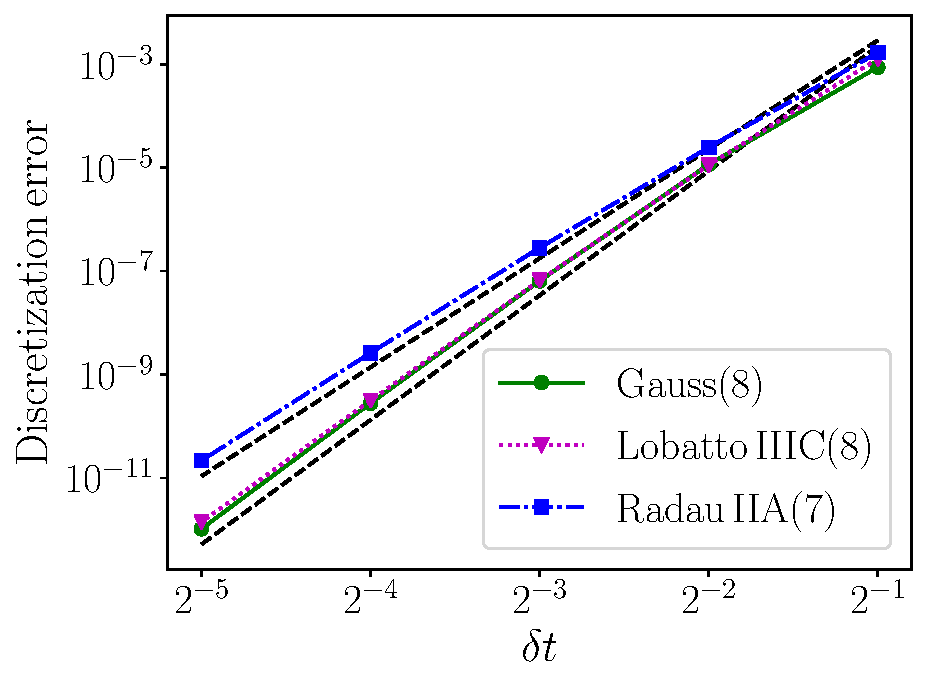
\includegraphics[width = 0.475\textwidth]{figures/FD_ex/errors_iters_18_38_27_d2_ex1.pdf}
\quad
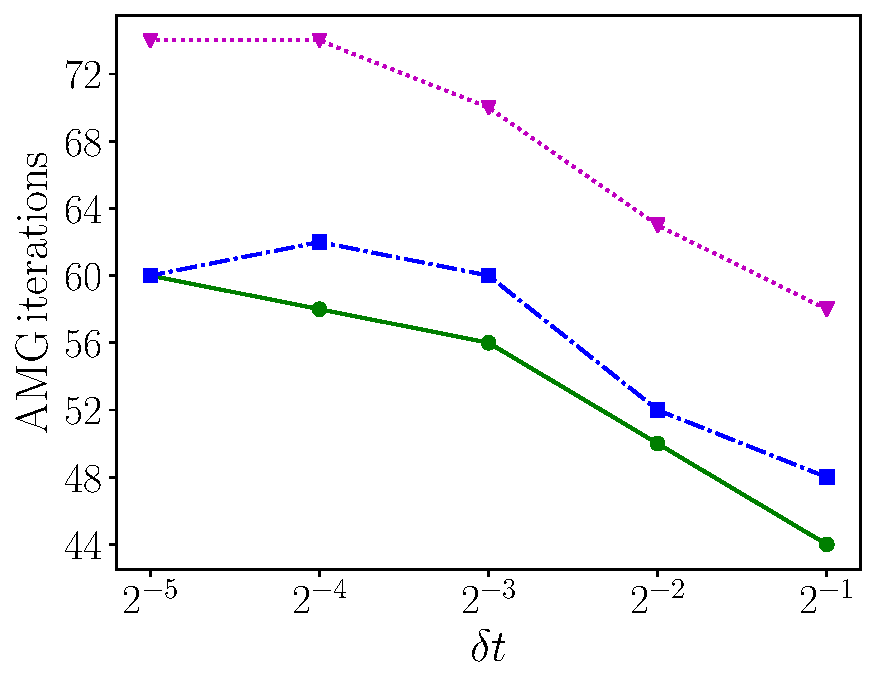
\includegraphics[width = 0.475\textwidth]{figures/FD_ex/amg_iters_18_38_27_d2_ex1.pdf}
}
\caption{Finite-difference advection-diffusion problem \eqref{eq:FD_ex}. At left, $L_{\infty}$-discretization errors at $t = 2$ as a function of time-step $\delta t$ for various discretizations of approximately 4th order (top) and 8th order (bottom). Black, dashed lines with slopes of three and four are shown (top), as are those with slopes of seven and eight (bottom). At right, average number of iterations per time step of the AMG preconditioner.
\label{fig:FD_ex}
}
\end{figure}



% ------------------------------------------------------------------------------------- %
% ------------------------------------------------------------------------------------- %
\subsection{Discontinuous Galerkin advection(-diffusion)}\label{sec:numerics:dg}

This section considers a more difficult advection-diffusion problem, discretized
using high-order discontinuous Galerkin finite elements. In particular, we demonstrate
the effectiveness and scalability of the new preconditioning on more complex flows and 
DG discretizations (\Cref{fig:ad_advdiff} and \Cref{sec:numerics:dg:adv}),
the reduction in computational work that can be achieved using large time steps and
very high-order integration (\Cref{sec:numerics:dg:adv}), and how
using multiple ``inner'' preconditioning iterations to approximate $\widehat{L}^{-1}$
(or even inner Krylov acceleration) can be important for the fast, scalable
application of IRK integration (\Cref{sec:numerics:dg:diff}).


\todo{Will, can you please add a problem/FEM discretization description here?}


\Cref{fig:ad_advdiff} plots the velocity field $\Omega(x,y)$ followed by the spatial
solution at five points in time (including the initial condition at $t=0$) using
diffusion coefficient $\kappa = 10^{-6}$.

% srun -n32 ./dg_adv_diff  -rs 3 -rp 1 -i 18 -o 4 -dt 0.1 -air 2 -tf 10 -e 1e-6 -nov
% dt = 0.1, hmin = 0.015625, hmax = 0.015625
% time order = 8, space order = 4
% time acc. = 1e-08, space acc. = 5.96046e-08
%
\begin{figure}[!htb]
  \centering
  \begin{subfigure}[b]{0.3\textwidth}
    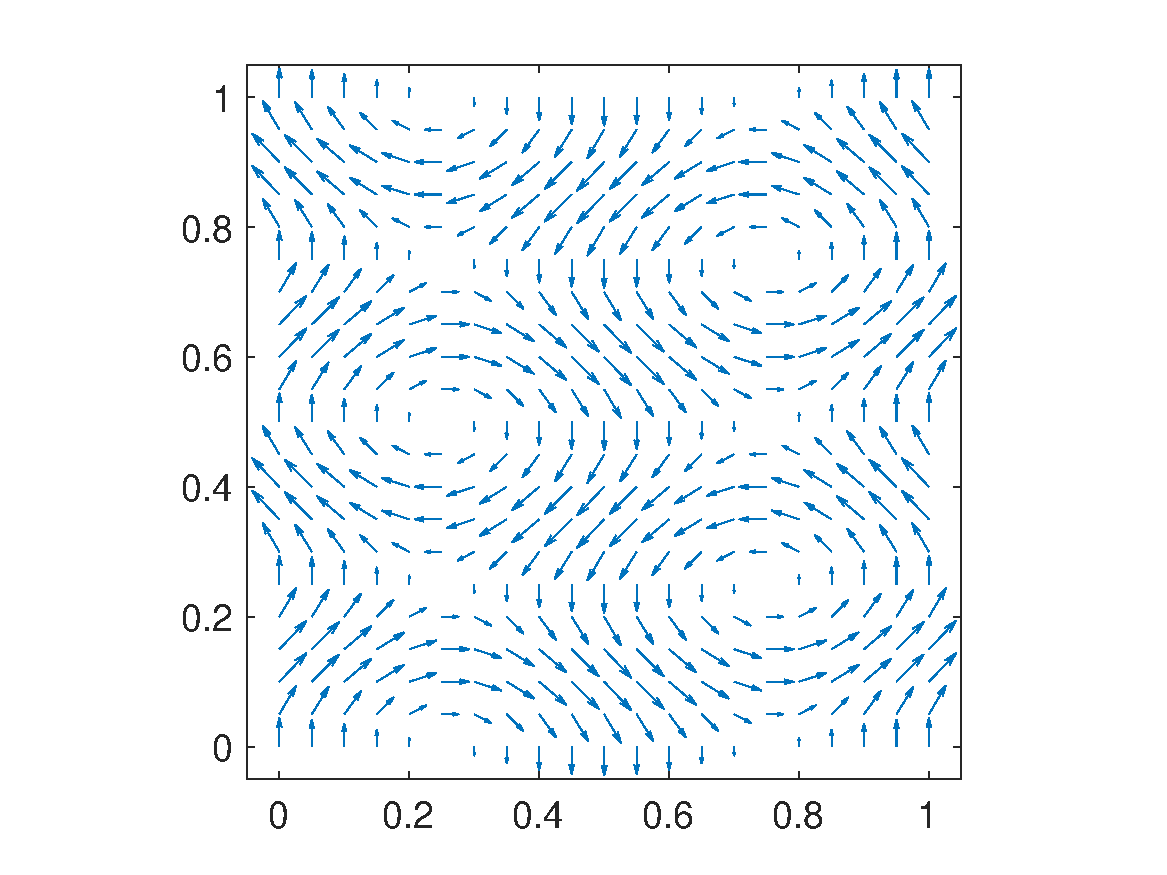
\includegraphics[width=\textwidth]{./figures/velocity_field.pdf}
    \caption{Velocity field}\label{fig:v}
  \end{subfigure}
   \begin{subfigure}[b]{0.3\textwidth}
    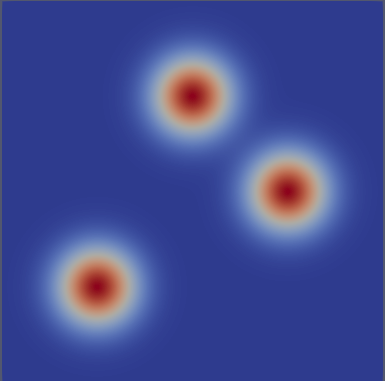
\includegraphics[width=\textwidth]{./figures/solution.0000.png}
    \caption{$t = 0$}
  \end{subfigure}
  \begin{subfigure}[b]{0.3\textwidth}
    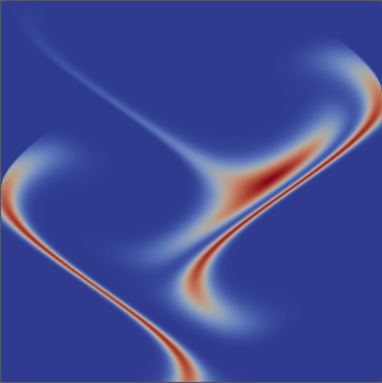
\includegraphics[width=\textwidth]{./figures/solution.0003.png}
    \caption{$t = 0.3$}
  \end{subfigure}
  \\\vspace{2ex}
   \begin{subfigure}[b]{0.3\textwidth}
    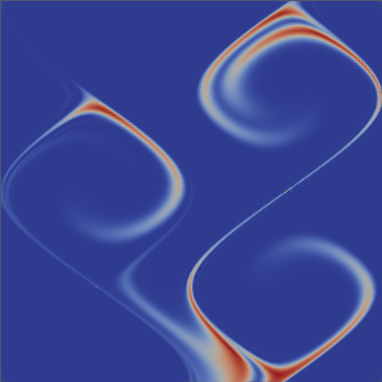
\includegraphics[width=\textwidth]{./figures/solution.0008.png}
    \caption{$t = 0.8$}
  \end{subfigure}
   \begin{subfigure}[b]{0.3\textwidth}
    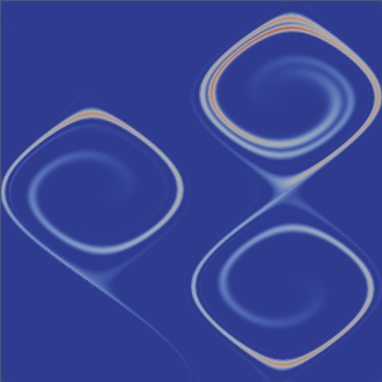
\includegraphics[width=\textwidth]{./figures/solution.0020.png}
    \caption{$t = 2.0$}
  \end{subfigure}
  \begin{subfigure}[b]{0.3\textwidth}
    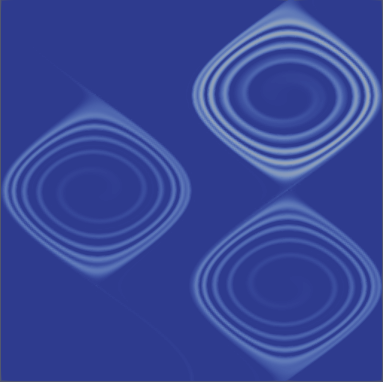
\includegraphics[width=\textwidth]{./figures/solution.0070.png}
    \caption{$t = 7.0$}
  \end{subfigure}
  \\\vspace{2ex}
      \caption{Advection-diffusion problem with velocity field shown in
      subplot (a) and the solution plotted for various time points from
      $t=0$ to $t = 7.0$ in subplots (b-f). Heatmap indicates solution in the
      2d domain, with blue $\mapsto 0$ and red $\mapsto 1$.}
  \label{fig:ad_advdiff}
\end{figure}

% ------------------------------------------------------------------------------------- %
\subsubsection{High-order \& advection-dominated}\label{sec:numerics:dg:adv}

First, we demonstrate high-order IRK integration applied to the advection-dominated
problem in \Cref{fig:ad_advdiff}, using AIR as a preconditioner for the linear
systems. AIR was originally designed for upwind DG discretizations of advection
and is well-suited for this problem. We use the \textit{hypre} implementation,
with distance 1.5 restriction with strength tolerance $\theta_R=0.01$, one-point
interpolation (type 100), Falgout coarsening (type 6) with strength tolerance
$\theta_C=0.1$, no pre-relaxation, and forward Gauss Seidel
post-relaxation (type 3), first on F-points followed by a second sweep on
all points. The domain is discretized using 4th-order finite elements on a
structured mesh, and the time step for each integration scheme is chosen
such that the spatial and temporal orders of accuracy match; for example,
for 8th-order integration we choose $\delta t = \sqrt{h}$, for mesh spacing
$h$, so that $\delta t^8 = h^4$. All linear systems are solved to a relative
tolerance of $10^{-12}$.

\Cref{fig:dg_o4_abs} shows the total numer of AIR iterations required to
compute one time step using six different Runge-Kutta schemes, from 4th
to 10th order, as a funciton of mesh spacing $h$. Note that as $h\to 0$,
there is only modest growth in the number of AIR iterations per time step,
indicating good (but not perfect) scalability.
Moreover, note that there is small growth in the number of iterations for
SDIRK4 as well (increasing from 20 to 25), which suggests the growth in
iteration count is due to imperfect scalability of AIR iterations rather
than the new IRK preconditioning.

\Cref{fig:dg_o4_rel} then shows the relative number of AIR iterations to
compute a given accuracy compared to SDIRK4. For example, if $h=0.01$,
then SDIRK4 uses $\delta t_4 = 0.01$ and Gauss8 uses $\delta t_8 =
\sqrt{0.01} = 0.1 = 10\delta t_4$, that is, $10\times$ less time steps to
achieve comparable accuracy. Note that as $h\to 0$, this factor becomes progressively
larger. For quite moderate $h$, we see how very high-order integration
can quickly lead to a reduction in total AIR iterations compared to a
standard SDIRK4 iteration. Gauss8, for example, requires $\approx 29\%$
of the total number of AIR iterations as SDIRK4 at $h =\delta t_4 = 1/256$,
and this ratio continues to decrease for smaller $\delta t$. Although this
does not account for additional setup time, where Gauss8 requires solving
two different linear systems and SDIRK4 only one, very high-order integration
permitted through the new preconditioning still offers the opportunity
for significant speedups.

%
\begin{figure}[!h]
  \centering
  \begin{subfigure}[b]{0.475\textwidth}
    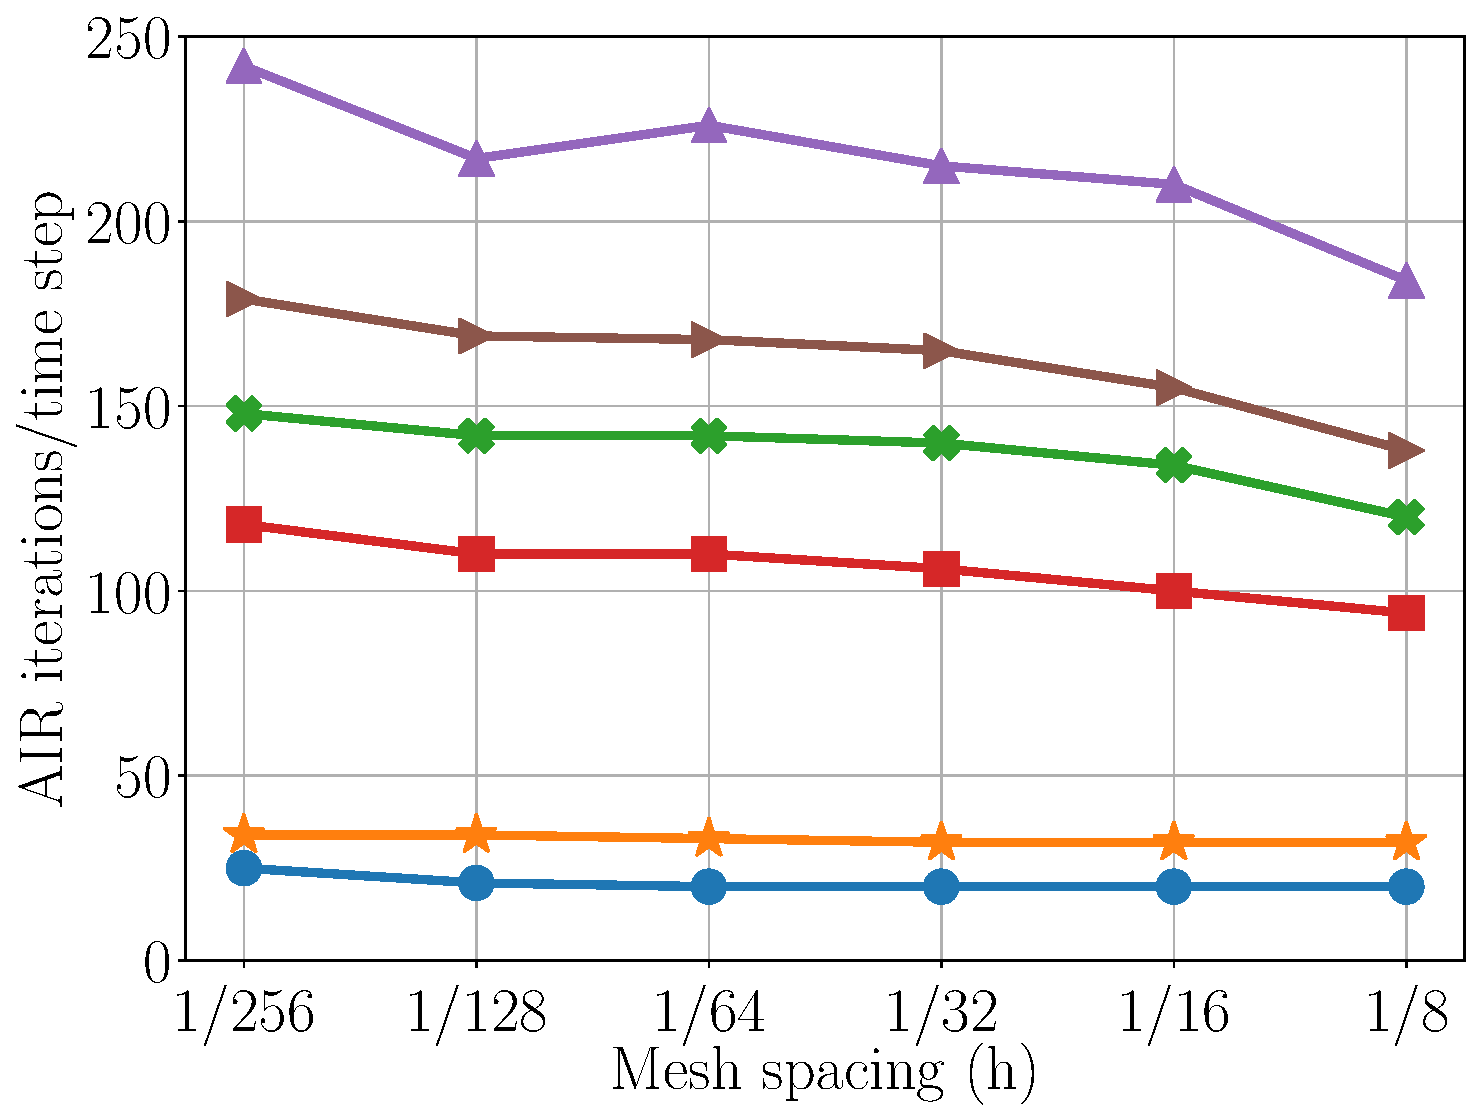
\includegraphics[width=\textwidth]{./figures/dg_advdiff_o4_1e-6.pdf}
    \caption{Total AIR iterations per time step}
	\label{fig:dg_o4_abs}
  \end{subfigure}
   \begin{subfigure}[b]{0.475\textwidth}
    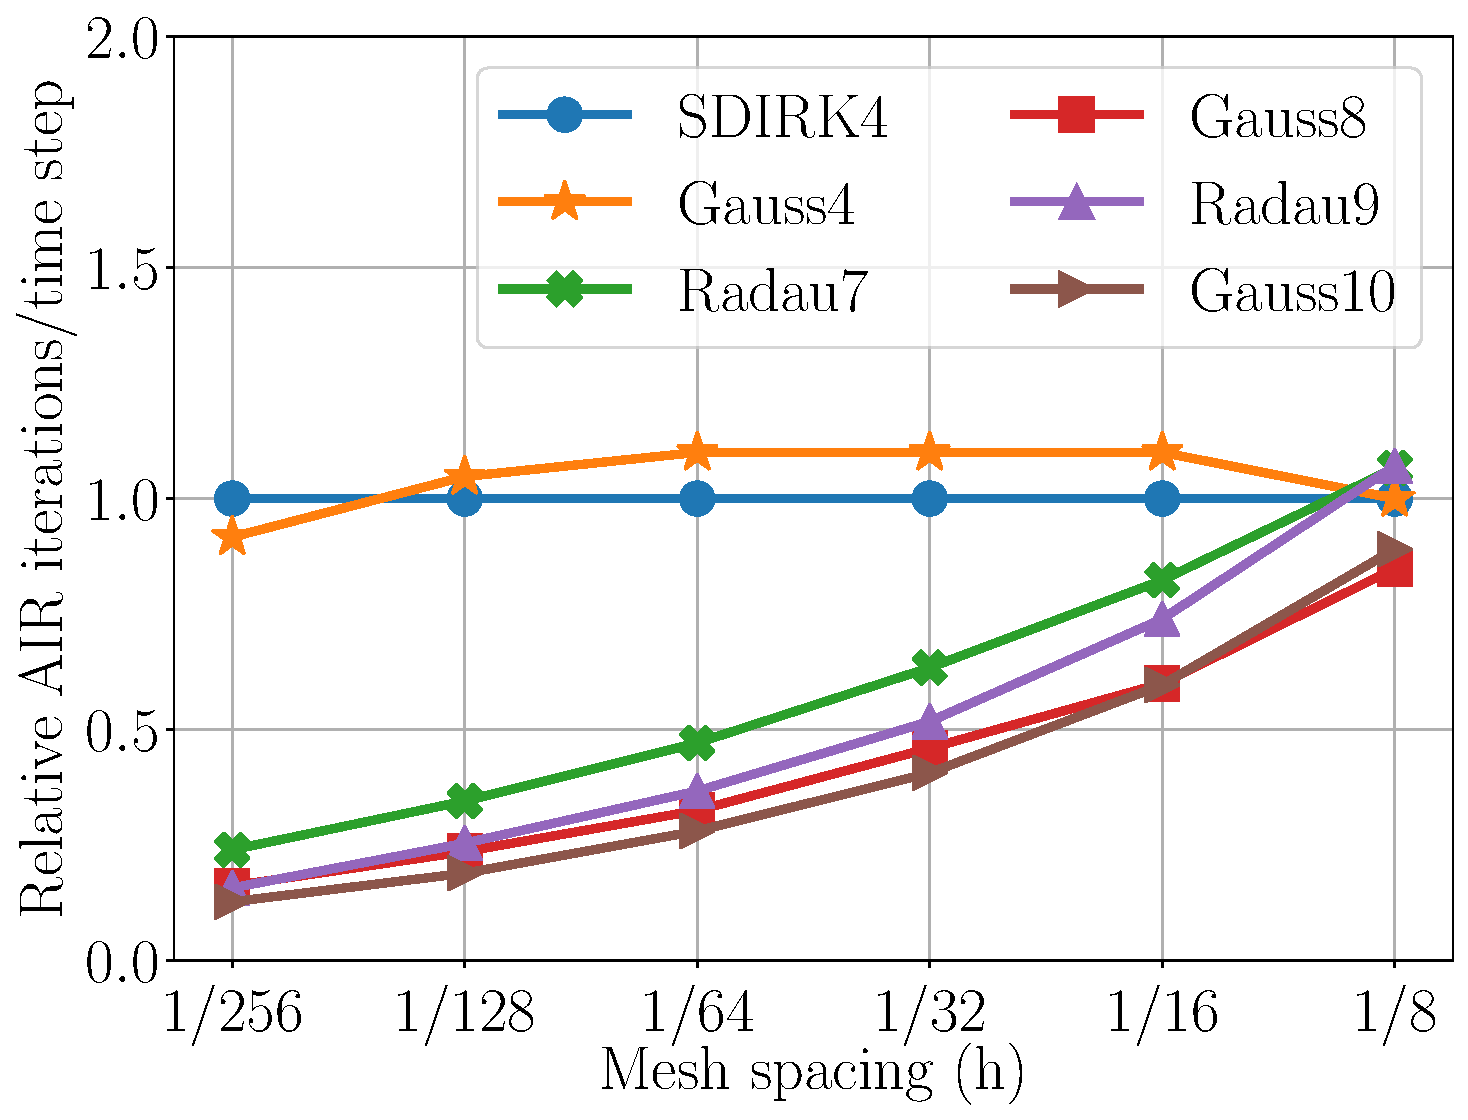
\includegraphics[width=\textwidth]{./figures/dg_advdiff_o4_1e-6_rel.pdf}
   \caption{AIR iterations relative to SDIRK4}
	\label{fig:dg_o4_rel}
  \end{subfigure}
\caption{}
  \label{fig:dg_o4}
\end{figure}
%


% ------------------------------------------------------------------------------------- %
\subsubsection{Diffusive problems and inner Krylov}\label{sec:numerics:dg:diff}

In \cite{AIR2}, AIR was shown to be effective on some DG advection-diffusion
problems, and classical AMG is known to be effective on diffusion-dominated
problems. However, the region of comparable levels of advection and diffusion
remains the most difficult from a multigrid perspective. We use this to 
demonstrate how methods developed here require a ``good'' preconditioner
for a backward Euler time step in order to converge on more general IRK
methods. However, ensuring a preconditioner is sufficiently good can be 
resolved analogous to block preconditioning techniques, where an inner
iteration is used that applies multiple AIR iterations as a single preconditioner.

Here we consider an analogous problem to above, but set the diffusion coefficient
to $\kappa = 0.01$. We use a mesh with spacing $h \approx 0.001$, 2nd-order
DG finite elements, a time step of $\delta t = 0.1$, and three-stage 6th-order
Gauss integration. Altogether, this yields equal orders of accuracy, with time and
space error $\sim10^{-6}$. FGMRES \cite{saad1993flexible} is used for the
outer iteration, which allows for GMRES to be applied in an inner iteration
as a preconditioner for $(\eta M - \mathcal{L})$. \Cref{fig:dg_o2} plots the
total number of AIR iterations per time step as a function of the number of
AIR iterations applied for each application of the preconditioner, using an
inner GMRES or an inner fixed-point iteration. 

Recall we have three stages, one of which is a single linear system coresponding
to a real eigenvalue, and the other corresponding to a pair of complex conjugate
eigenvalues, which we precondition as in \Cref{sec:solve}. The latter ends up being
the more difficult problem to solve -- using one AIR iteration as a preconditioner,
the outer FGMRES iteration for the complex conjugate quadratic does not converge in
1000 iterations. If two AIR iterations with GMRES are used as a preconditioner,
the FGMRES iteration converges in approximately 130 iterations, each of which
requires two applications of GMRES preconditioned with two AIR iterations,
yielding just over 500 total AIR iterations to converge. Further increasing
the number of AIR iterations per preconditioning yields nice convergence
using inner fixed-point or GMRES, with 150 and 112 total AIR iterations per
time step, respectively. 

\begin{figure}[h!]
\centering
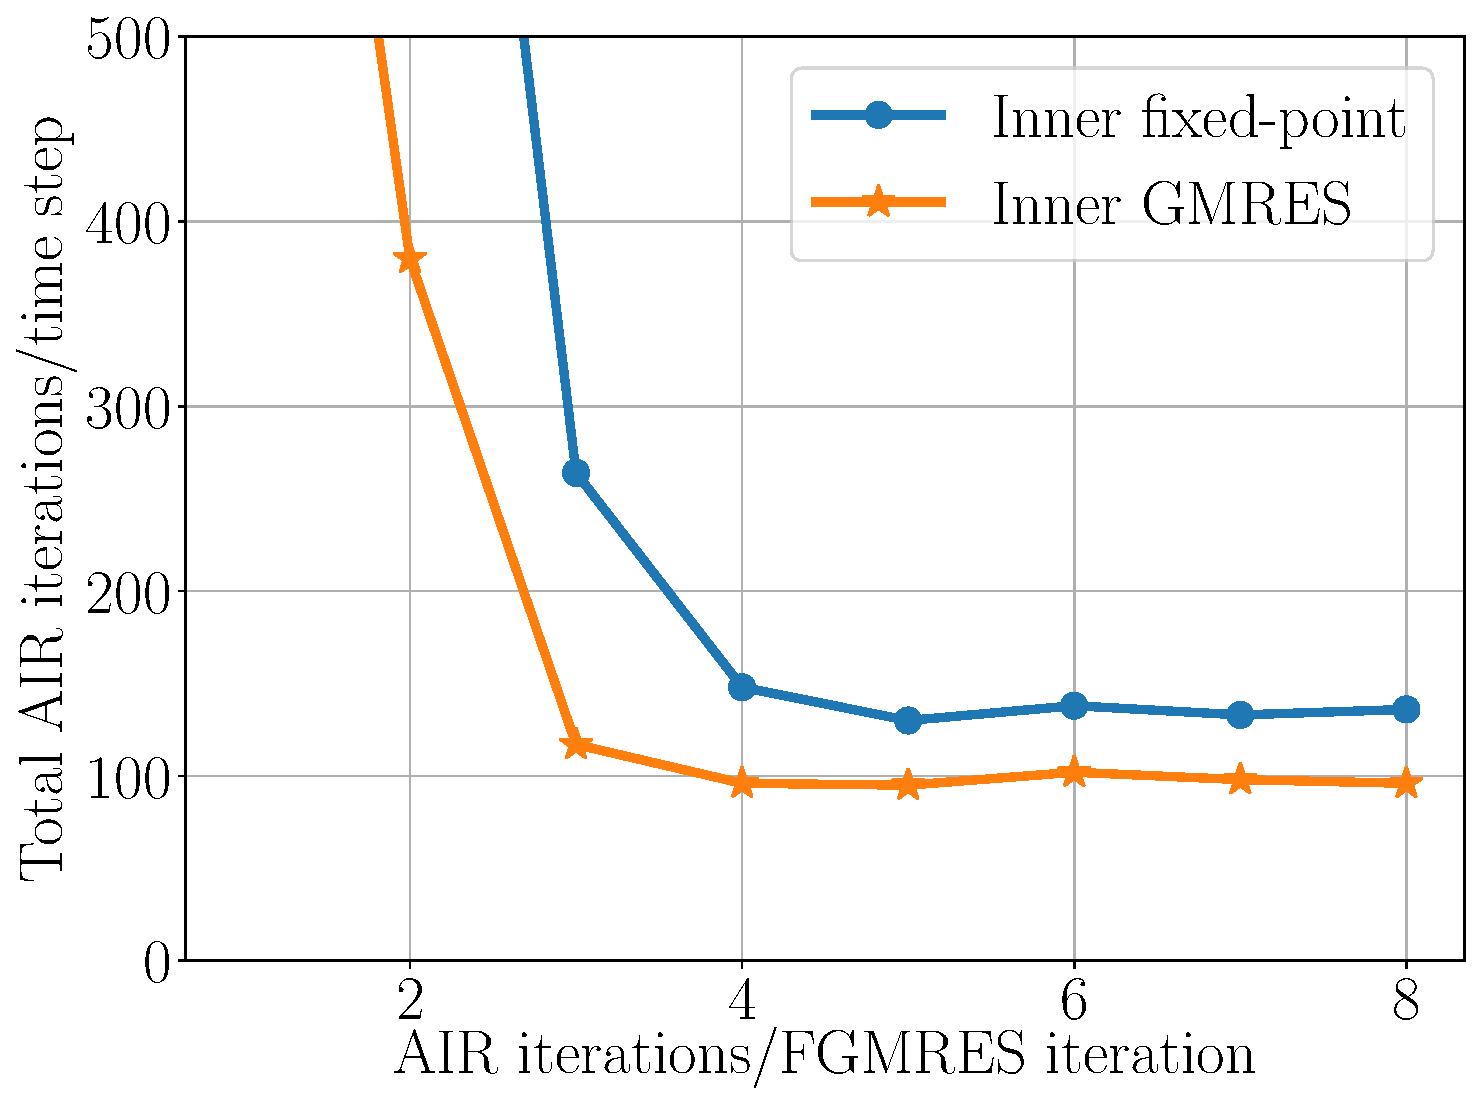
\includegraphics[width = 0.55\textwidth]{./figures/dg_advdiff_o2_1e-2.pdf}
\caption{AIR iterations per time step as a function of the number of
AIR iterations applied for each application of the preconditioner.}
\label{fig:dg_o2}
\end{figure}




% ------------------------------------------------------------------------------------- %
% ------------------------------------------------------------------------------------- %
\subsection{High-order matrix-free diffusion}






% ------------------------------------------------------------------------------------- %
% ------------------------------------------------------------------------------------- %
% ------------------------------------------------------------------------------------- %
\section{Conclusions}\label{sec:conc}

This paper introduced a theoretical and algorithmic framework for the fast, parallel
solution of fully implicit Runge-Kutta methods in numerical PDEs (without algebraic
constraints). A field-of-values analysis is derived to guarantee rapid Krylov
convergence...\todo{finish}

% ------------------------------------------------------------------------------- %
\bibliographystyle{siamplain}
\bibliography{refs2.bib}


\end{document}
